\documentclass[supercite]{HustGraduPaper}

\title{区块链公有链交易监控与溯源系统设计与实现}
\author{Alaric}
\school{计算机科学与技术}
\classnum{CS18XX}
\stunum{U2018XXXXX}
\instructor{XXX}
\date{2022年6月1日}

\usepackage{algorithm}
\usepackage{algpseudocode}
\usepackage{amsmath}
\usepackage{amsthm}
\usepackage{framed}
\usepackage{mathtools}
\usepackage{subcaption}
\usepackage{xltxtra}
\usepackage{bm}
\usepackage{tikz}
\usepackage{hyperref}
\usepackage{minted}
\usetikzlibrary{shapes,positioning}
\usepackage{tikzscale}
\usepackage{pgfplots}
\usepackage[perpage]{footmisc}
\pgfplotsset{compat=1.16}

\newcommand{\cfig}[3]{
  \begin{figure}[htb]
    \centering
    \includegraphics[width=#2\textwidth]{images/#1.tikz}
    \caption{#3}
    \label{fig:#1}
  \end{figure}
}
\newcommand{\sfig}[3]{
  \begin{subfigure}[b]{#2\textwidth}
    \includegraphics[width=\textwidth]{images/#1.tikz}
    \caption{#3}
    \label{fig:#1}
  \end{subfigure}
}
%\sxfig[name][width][title]{
%  
%}
\newcommand{\sxfig}[4]{
  \begin{subfigure}[b]{#2\textwidth}
    #4
    \caption{#3}
    \label{fig:#1}
  \end{subfigure}
}
\newcommand{\xfig}[3]{
  \begin{figure}[htb]
    \centering
    #3
    \caption{#2}
    \label{fig:#1}
  \end{figure}
}

\newcommand{\rfig}[1]{\autoref{fig:#1}}
\newcommand{\ralg}[1]{\autoref{alg:#1}}
\newcommand{\rthm}[1]{\autoref{thm:#1}}
\newcommand{\rlem}[1]{\autoref{lem:#1}}
\newcommand{\reqn}[1]{\autoref{eqn:#1}}
\newcommand{\rtbl}[1]{\autoref{tbl:#1}}

\algnewcommand\Null{\textsc{null }}
\algnewcommand\algorithmicinput{\textbf{Input:}}
\algnewcommand\Input{\item[\algorithmicinput]}
\algnewcommand\algorithmicoutput{\textbf{Output:}}
\algnewcommand\Output{\item[\algorithmicoutput]}
\algnewcommand\algorithmicbreak{\textbf{break}}
\algnewcommand\Break{\algorithmicbreak}
\algnewcommand\algorithmiccontinue{\textbf{continue}}
\algnewcommand\Continue{\algorithmiccontinue}
\algnewcommand{\LeftCom}[1]{\State $\triangleright$ #1}

\newtheorem{thm}{定理}[section]
\newtheorem{lem}{引理}[section]

\colorlet{shadecolor}{black!15}

\theoremstyle{definition}
\newtheorem{alg}{算法}[section]

\def\thmautorefname~#1\null{定理~#1~\null}
\def\lemautorefname~#1\null{引理~#1~\null}
\def\algautorefname~#1\null{算法~#1~\null}

\tikzstyle{inout}=[trapezium, trapezium left angle=60, trapezium right angle=120, draw] %%输入输出框
\tikzstyle{end}=[rectangle, rounded corners, draw]   %%教材上的起止框
\tikzstyle{endn}=[rounded rectangle, draw]   %%新版的起止框
\tikzstyle{exec}=[rectangle, draw]    %%执行框 execute
\tikzstyle{decide}=[kite, kite vertex angles=120, draw]   %%判断框
\tikzstyle{box}=[rectangle, draw]
\tikzstyle{vbox}=[rectangle, draw, text width = 1em]
\captionsetup{justification=centering}
\begin{document}

\maketitle

\statement

\clearpage

\pagenumbering{Roman}

\begin{cnabstract}{加密货币;去匿名化;比特币;区块链}

  近年来,随着计算机设备运算能力的进步和区块链技术的蓬勃发展,以区块链作为核心技术并利用工作量证明机制完成共识机制的加密货币得到了广泛应用,加密货币成为了一种事实上流行的支付工具。然而加密货币天然的匿名属性也广受犯罪分子的青睐,被频繁用于洗钱、赌博与非法黑市交易,这对国家的网络安全发展构成了严重的危害。因此,对公有链上的网络节点及其拓扑进行探测与分析,并通过对链上实时发生的交易进行追踪和去匿名化工作实施对加密货币交易监管是一个亟待解决的问题。

  本文从对加密货币交易监管的需求出发,设计并实现了一个区块链公有链交易监控与溯源系统,系统可以利用加密货币对等网络交易信息的传输,对其对等网络中的消息进行解析和处理,对交易信息去匿名化;同时系统采取任务分配和分布式部署机制,使用后端节点对不同节点获取的去匿名化消息进行分析和存储;系统提供了一个客户端,可供政府工作人员操作,对区块链上可疑的交易进行监管和追踪。

  通过测试表明,该系统成功实现了比特币的网络传输协议,连接入其网络获取交易信息,经过去匿名化分析后存储;系统提供了在时间、IP地址和交易标识符三个不同维度查询交易信息的功能,在一定程度上改善了加密货币缺乏系统性监控溯源工具的现状。整个系统分为三大模块:交易监控溯源模块、后端存储管理模块和客户端管理和展示模块;应用到的技术有:远程过程调用、WPF、Kitex以及零拷贝数据处理。


\end{cnabstract}

\begin{enabstract}{Cryptocurrency, Deanonymization, Bitcoin, Block chain}

  In recent years, with the advancement of the computing power of computer equipment and the vigorous development of blockchain technology, cryptocurrencies that take blockchain as the core technology and use the proof-of-work mechanism to complete the consensus mechanism have been widely used, and cryptocurrencies have become a kind of popular payment tool. However, the anonymous natural property of cryptocurrencies is also widely favored by criminals. It is frequently used for money laundering, gambling, and illegal black market transactions, which seriously harms the development of the country's cyber security. Therefore, it is an urgent problem to detect and analyze the topology of the cryptocurrency network and implement a supervisor of cryptocurrency by tracking and de-anonymizing transactions that occur on the chain.

  This paper designs and implements a blockchain public chain transaction monitoring and traceability system starting from the demand for cryptocurrency transaction supervision. The system can use the transmission of cryptocurrency peer-to-peer network transaction information to parse the messages in its peer-to-peer network and process to de-anonymize it; at the same time, the system adopts task allocation and distributed deployment mechanism and uses back-end nodes to analyze and store de-anonymized messages obtained by different nodes; the system provides a client for civil servants operation to monitor and track suspicious transactions on the blockchain.

  The test shows that the system successfully implements the Bitcoin network transmission protocol, connects to its network to obtain transaction information, and stores it after de-anonymization analysis; the system provides three dimensions of time, IP address and transaction identifier to query de-anonymized transactions, which has improved the status quo of the lack of systematic monitoring and traceability tools for cryptocurrencies to a certain extent. The whole system is divided into three modules: transaction monitoring module, back-end module and client module; the applied technologies are remote procedure call, WPF, Kitex and zero-copy data processing.

\end{enabstract}

\tableofcontents[level=2]
\clearpage

\pagenumbering{arabic}

\section{绪论}

本章首先介绍了区块链技术以及以区块链为核心技术蓝本的加密货币的应用前景,阐述了当前加密货币对社会稳定造成的风险,随后分析了监控加密货币公有链交易面临的挑战和技术发展趋势,介绍了国内外在加密货币去匿名化领域的相关研究工作,并对本文的主要研究内容及工作意义作了具体说明。

\subsection{课题背景}

\subsubsection{研究背景和趋势}

区块链是一种利用哈希算法、Merkle树、工作量证明以及点对点网络(Peer to Peer,P2P)的可信分布式数据库\cite{何蒲2017区块链技术与应用前瞻综述},这种新型分布式数据库,可以在互不信任的环境中实现不依靠中介的可靠交易;与传统数据库技术相比,区块链技术具有防伪防篡改、智能合约实现等特点,被誉为引领社会变革的新技术\cite{陈伟利2018区块链数据分析}。以区块链作为核心技术的加密货币有着高度去中心化的特征,能够通过运用数据加密、时间戳、分布式共识和经济激励等手段,在节点无需互相信任的分布式系统中实现基于去中心化信用的点对点交易、协调与协作\cite{袁勇2016区块链技术发展现状与展望}。自2008年中本聪发布比特币白皮书\cite{nakamoto2008bitcoin}以及其次年启动比特币项目开始,相当大数量的金融交易借助了如井喷爆发的各类加密货币金融系统进行,作为加密货币实例化先驱的比特币,平均每天有约22\textasciitilde27万笔交易被写入分布式区块链数据库,其每天的交易价值在200\textasciitilde600亿美元间波动\footnote{数据来源:\url{https://bitinfocharts.com/bitcoin/}。}。

然而加密货币天然的匿名属性也广受犯罪分子的青睐,被频繁用于洗钱、赌博与非法黑市交易\cite{moser2013inquiry,conti2018survey},这对国家的网络安全发展构成了严重的危害。区块链公有链系统去中心、自治化、强匿名等特性使得基于公有链系统所发生的网络安全事件和网络犯罪行为难于被监测与溯源,导致政府和机构无法对公有链系统进行有效的监管,大大制约了公有链的应用范围和应用场景。因此,对公有链上的网络节点及其拓扑进行探测与分析,并通过对链上实时发生的交易进行追踪和去匿名化工作实施对加密货币交易监管是一个急需解决的问题。

\subsubsection{面临的问题和挑战}

\textbf{从对等网络中找到信息发布源}\ 与传统的金融系统不同,得益于区块链可信式分布数据库的高度去中心化,比特币等加密货币不依靠中心化的记账系统,交易信息通过对等网络在整个货币网络中扩散。即使交易信息最终可以在区块链网络上轻松获取到,由于交易信息仅包含与交易相关的支出和收取方账户与电子签名等信息,无法从高度匿名化的交易信息中获取有效真实信息。如何利用对等网络中消息的传递有效获取到消息传播源的真实地址,成为区块链上交易溯源和监控的重要挑战。

\subsection{国内外研究现状}
加密货币网络层常有两类模型\cite{wu2021analysis}。一种与寻常的银行账户模型类似,另一种是以比特币为代表的UTXO模型,这种加密货币的区块中存储的只有交易信息,任何一个交易,它总是由若干个输入(Input)和若干个输出(Output)构成,一个输入指向的是前面区块的某个输出,只有矿工奖励的铸币交易没有输入,只有输出。还没有被下一个交易花费的Output被称为UTXO(Unspent TX Output),即未花费交易输出。这种模型的交易模型和账户模型有所不同,它并没有账户这个说法,只有UTXO,一个地址持有的加密货币即为账号地址的UTXO之和。
\xfig{utxo}{UTXO交易模型}{
  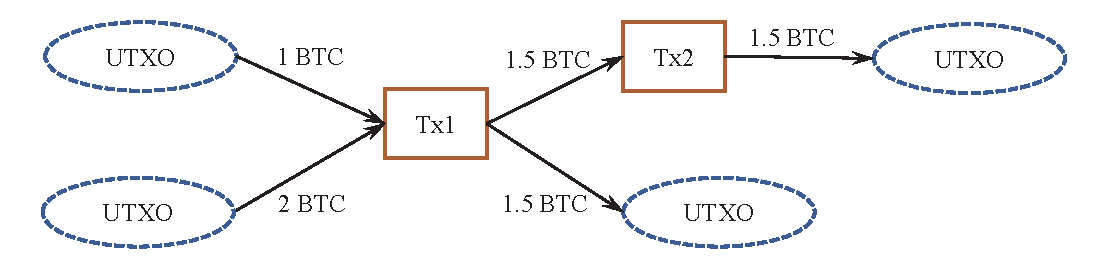
\includegraphics[width=0.75\textwidth]{images/1.1-utxo.ps} 
}

围绕比特币等加密货币的网络模型构建的加密货币的去匿名化工作基本可分为两个方向:一种是基于网络传输的溯源技术,可以利用点对点信息泛洪传递本身,使用受控节点获取信息,通过一定的传播源估计算法分析其信息在网络中的传输途径,进而直接获取交易始发节点的IP地址,这种方式需要使用大量带宽和算力连接至整个对等网络,但获取的信息可以直接对交易和地址去匿名化;另一种是基于历史数据的交易分析技术,通过分析存储在分布式数据库中的历史交易信息,对不同地址间的交易进行行为分析,从而获取匿名用户的交易规律,这种方式的算力需求较小,且往往可以利用深度学习等技术使用通用计算平台迅速分析出交易行为,但得到的结果只是匿名用户的行为规律,无法直接获取交易和账户持有者的真实信息。虽然通过分析互联网上公开的讨论信息,将互联网公开平台上的用户、交易行为描述等与匿名的交易账户、交易行为进行联系和候选分析也能完成去匿名化,但这种方式容易被加密货币用户使用混币策略\cite{bonneau2014mixcoin}和一次性地址策略绕过。


\subsubsection{基于网络传输的溯源技术}
Biryukov\cite{biryukov2014deanonymisation}等人利用比特币对等网络中节点发现的协议,提出了一种通过向比特币服务器建立多个连接,唯一地识别比特币客户端的一组入口节点的方法\footnote{默认情况下,比特币节点客户端试图保持8个向外建立的连接,同时服务端可以监听多达117个传入连接。该文中将客户端建立连接的8个节点称为入口节点。},并提出只要监控者从2-3个入口节点收到交易,他就很有可能将交易确定到特定客户端。同时成功去匿名化的交易可以反过来帮助跟踪入口节点集中的动态变化,以保持客户端标识的最新。对整个比特币网络进行去匿名化的成本并不高\footnote{2014年比特币用户数约150万,实验结果表明当时平均服务端数目约为8000个,客户端数约为100000个,监控成本约1\textasciitilde 1.5万元每月。}。

Fanti\cite{fanti2017anonymity,fanti2017deanonymization}等人提出对用户进行去匿名化的问题在数学上等同于在给定传播的部分观察结果的情况下推断图上随机传播过程的来源。对于传播源的估计,Shah等人提出了谣言中心性检测\cite{shah2012rumor},Zhaoxu等人提出了谣言中心性在多个观察者下算法和限制\cite{wang2014rumor};Zhukai等人提出了一种高鲁棒性的具有稀疏观测的信息源估计器\cite{zhu2014robust}。而Fanti等人针对比特币等加密货币对等网络的特点,针对不同的传播策略提出了首时间戳估计、报告中心估计和球中心估计,并给出了估计方法的准确度下界。估计方法的准确度下界和在比特币网络拓扑\cite{miller2015discovering}上的测试结果表明:比特币的泛洪协议有较差的匿名性,且比特币社区把对等网络交易信息泛洪协议从涓滴传播到扩散传播的改进无助于改善其匿名性,可以通过在比特币网络上布置大量受控的对手节点对比特币地址和IP地址(Internet Protocol Address)进行关联,完成比特币交易的去匿名化。

高峰\cite{高峰2018轻量级比特币交易溯源机制}等人提出提出了一种轻量级比特币交易溯源机制,可以将比特币地址和始发服务器节点的IP地址关联,并通过实验验证了这种轻量级溯源机制可以对非可控比特币服务器节点开展交易溯源。这种关联关系可以用于发现恶意使用比特币交易的用户身份信息、追踪资金流向,为解决比特币勒索等非法比特币交易问题提供一种新的思路。


而为了提升比特币网络的吞吐量和匿名性,Naumenko等人提出使用一种名为Erlay\cite{naumenko2019erlay}的新的传播协议替代先前的协议,通过利用 pinsketch 算法\cite{2008Fuzzy}计算得出的草图(sketch),高效的找出 2 个节点之间交易集合的差异,然后进行传输,这种无需通过询问交易ID(Identifier,标识符)的方式,能有效的降低交易信息泛洪传播使用的带宽,同时使得传播源估计难以进行。

\subsubsection{基于历史数据的交易分析技术}

Fleder\cite{fleder2015bitcoin}等人分两部分构建了一个比特币交易图标注系统:他们首先了开发一个从公共论坛收集比特币地址的系统,随后引入了一种使用不完整的事务信息将用户与交易匹配的机制,通过对网页中信息的收集进行分析,将网页中非匿名个体的对交易行为的描述解析,通过汇率计算对应比特币价值并通过分析获取交易可能发生的时间,生成候选交易匹配和相关的匹配概率,将交易与实体关联。同时他们还提出了一个图形分析框架,能够跟踪和聚类用户活动。通过利用通过网络搜集的论坛和比特币交易账本的公开信息来源,证明了比特币交易网络并非完全匿名。

郭文生\cite{郭文生2021基于机器学习的比特币去匿名化方法研究}等人提出一种联合特征构造方法并构建随机森林与Softmax相结合的分类模型,通过比特币交易系统中比特币地址聚类的关联规则,在地址集群海量的链上交易数据中抽取与地址集群相关的交易特征。设计比特币地址身份识别机制中的特征提取与融合方案,采用机器学习的方法有效地识别比特币地址的身份。

李南铮\cite{李南铮2021比特币的网络交易特征分析及实体识别算法研究与设计} 提出了一种利用关联特征进行实体识别分类的方法,从比特币地址自身的多交易关联特性作为切入点,对比特币进行实体识别;同时与Fleder的思路一致,在该文中也采用了从互联网公开社交平台爬取信息进行标注对实体识别进行验证的方法。该算法和系统能有效提升实体识别的性能,为监管部门大规模部署对比特币等加密货币的监控提供了可能。

黄一\cite{黄一2021以太坊平台实体识别系统的研究与设计} 针对以太坊模型的加密货币的实体识别的数据处理和分析过程,提出了启发式方法、追踪溯源算法、机器学习识别三种去匿名化方法,借助用户资金来源去向识别用户交易行为,量化用户合规程度。通过识别账户的行为辨识账户持有者的合规性,从而给个人用户提供风险规避的依据、给监管部门提供一定的量化监管和分析能力。

钱智成\cite{钱智成2021比特币交易行为分析系统研究与设计} 认为传统实体识别的或通过启发式方法,或通过特征工程,忽略了比特币等加密货币交易UTXO模型可构成有向无环图的特性。该文通过利用比特币交易的图结构特征,提出了一种利用时序信息的识别方法和一种利用图神经网络的识别方法,提升了实体识别模型在比特币上的表现,其实现的比特币交易行为分析系统能对资金来源去向进行一定的去匿名化,为监管部门取证提供便利。

\subsection{研究目的和主要内容}
理解区块链网络中节点探测与拓扑分析的原理,熟悉区块链网络协议中交易信息扩散的过程,学习对等网络中解决去匿名化问题的手段,研究大规模公有链网络下区块链交易的追踪与溯源方法。进而在此基础上,实现一个区块链公有链交易监控与溯源系统,使得系统具有区块链网络交易节点拓扑结构的构建与分析、交易行为的监控与溯源的功能。

详细的工作包括:

1、根据虚拟货币交易特性,抽象出一套与具体货币类型无关的信息传递通信接口,根据比特币社区提供的通信协议,实现基于比特币的通信接口。

2、根据文献中提出的传播源估计方法,基于信息传递接口实现基于这些算法的嗅探节点。

3、根据文献中提出的传播源估计方法所需的多嗅探节点的特性,实现用于配置监控节点任务和交换信息的上位节点,并实现监控节点与上位节点间的RPC网络通信。

4、实现上位节点对监控节点汇报来的监控结果的存档,并实现这些监控信息获取的HTTP接口。

5、实现一个用于展现实时监控结果的最终用户界面。


\subsection{课题来源}
该课题是本人在第七学期(大四上学期)在毕业设计选题系统上所选择的课题,该课题由李瑞轩老师带领研究,主要研究区块链公有链交易监控与溯源工作,这是区块链里一项具有挑战性的工作。
\subsection{论文结构}

本论文共分为六个章节:

第一章,首先介绍了加密货币的发展现状及其导致的社会问题,阐述了开发一个区块链公有链监控与溯源系统的必要性;随后从比特币为代表的UTXO模型出发,介绍了不同模型下加密货币去匿名化的两个方向,以及综述了国内外在这两个方向上做的前瞻性研究,为本文开发一个区块链公有链监控与溯源系统给出了理论基础。

第二章,将首先分析开发一个区块链公有链监控与溯源系统的项目需求,随后围绕技术可行性和社会可行性两个方面着手进行可行性分析,根据需求选择了合适的开发工具以及介绍了选取这些开发工具的原因;最后简要介绍了开发该区块链公有链监控与溯源系统可能需要的理论前提,为详细设计区块链公有链监控与溯源系统各个模块功能提供方案和技术基础。

第三章,根据课题需要,将首先确定区块链公有链监控与溯源系统的网络架构,然后对系统进行自顶向下的设计,将对系统的客户端模块、Peer交互模块、后端模块和监控嗅探模块的功能做出具体安排,为开发实现区块链公有链监控与溯源系统提供蓝图。

第四章,在整个系统的设计介绍完成之后,开始说明区块链公有链监控与溯源系统的具体实现细节,比如基于比特币通信协议的Peer交互模块的实现、监控嗅探模块核心工作流程等等,介绍了系统的实现方案。

第五章,着重进行单元测试和系统测试结果的过程和结果展示,主要包括测试技术的介绍、关键模块的测试用例举例和系统的实现效果展示。

第六章,会对整个区块链公有链监控与溯源系统的实现进行总结,总结其已经实现的所有功能,并在论文的最后展望本系统下一步的发展计划。

\newpage
\section{方案论证}
本次毕业设计旨在实现一个完整全面的区块链公有链交易监控与溯源系统,使得系统具有区块链网络交易节点拓扑结构的构建与分析、交易行为的监控与溯源的功能。本章将从需求分析出发,分析系统需要具备的监控嗅探、存储管理和客户端操作三大模块的基本功能需求;经可行性分析论证后选取合适的开发技术工具,随后简述系统运用到的算法基础,对整个监控系统的分析设计做出完整的说明和论证。
\subsection{系统需求分析}\label{sec:demands}
区块链公有链交易监控与溯源系统的主要功能有:分析区块链网络交易节点拓扑、监控并溯源加密货币交易以及对监控的信息进行查询;大多数的基于网络拓扑结构的去匿名化监控手段通过加密货币网络中的受控制的超级节点完成:这个节点可以与每个加密货币服务器建立多个连接,每个连接来自不同的(IP地址,端口)元组。由于当前加密货币有着种类繁多、应用广泛的特点,仅仅在单台计算机设备上完成对加密货币的监控是难以进行的。因此该系统需要和加密货币类似的思路,采取分布式部署的方式。在这个前提下,需要完成三个功能来构建整个监控系统:
%\xfig{sniffer}{监控嗅探功能树}{
%  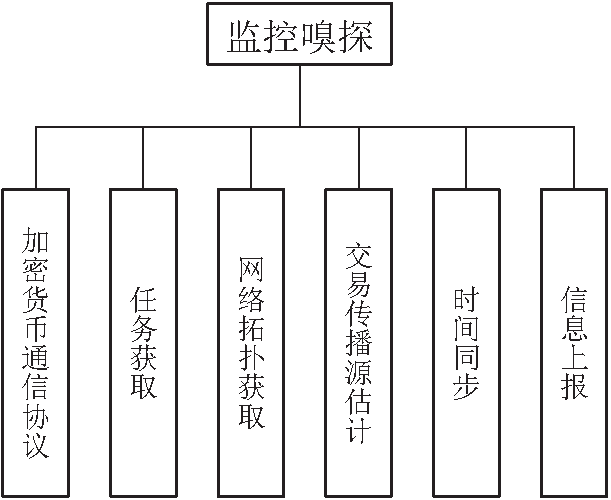
\includegraphics[width=0.6\textwidth]{images/2.1-sniffer.ps} 
%}

\textbf{监控嗅探功能}\ (见\rfig{sniffer})系统需要实现加密货币通信协议,从后端获取监控分析的任务,根据任务指定的加密货币约定的固定“种子DNS”获取点对点网络的初始节点列表,连接至初始化节点并在线程池中获取加密货币节点给出的邻节点信息,连接至整个加密货币网络的一个子图,直至设定的可连接数上限。随后根据连接到的加密货币网络节点传来的交易信息,借助不同的传播源估计算法给出当前子图中可能的交易始发节点信息,上报到系统后端进行存储。在监控嗅探进行的同时需要和系统后端进行周期性通信,通过时间同步算法抹除不同节点间的系统运行时间差异,保证上报信息时间戳足够准确。

\textbf{后端存储管理功能}\ (见\rfig{store})系统需要综合不同节点给出的交易来源IP结论给出最优结果,并将所有结果和最终估计写入数据库,并提供HTTP JSON接口功能给客户端查询;提供保存各个监控节点的任务列表的功能,在监控嗅探节点获取任务时给出任务分配;提供时间同步的服务端功能,在监控嗅探节点给出查询同步时间包后返回自身的时间戳。

\textbf{客户端操作呈现功能}\ (见\rfig{client})系统需要给最终用户提供一个可视化的操作界面,用于修改节点任务列表、分别按时间查询最终各个估计算法给出的可能的加密货币交易信息的去匿名化结论、按交易ID查询所有节点的报告信息以及按IP地址查看涉及的所有交易,在一定程度上提供一个完整的加密货币监控与溯源系统的用户交互逻辑。
\xfig{system-requirements}{系统需求功能树}{
  \begin{subfigure}[b]{0.54\textwidth}
    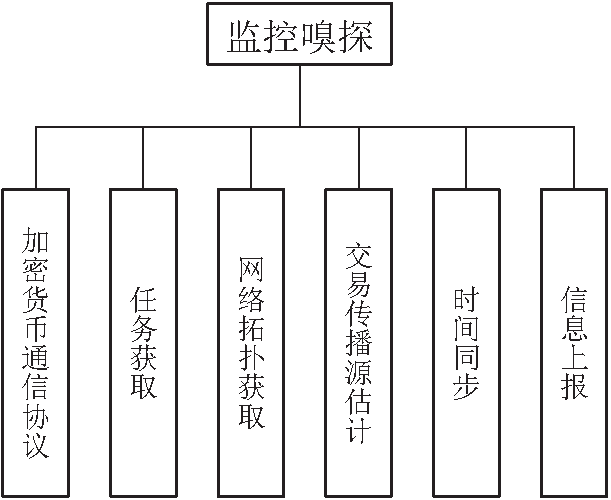
\includegraphics[width=\textwidth]{images/2.1-sniffer.ps}
    \caption{监控嗅探功能树}
    \label{fig:sniffer}
  \end{subfigure}
  \begin{subfigure}[b]{0.54\textwidth}
    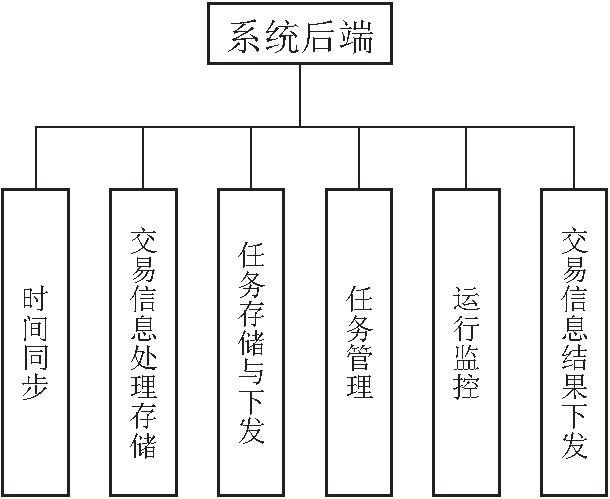
\includegraphics[width=\textwidth]{images/2.1-backend.ps}
    \caption{后端存储管理功能树}
    \label{fig:store}
  \end{subfigure}
  \begin{subfigure}[b]{0.4\textwidth}
    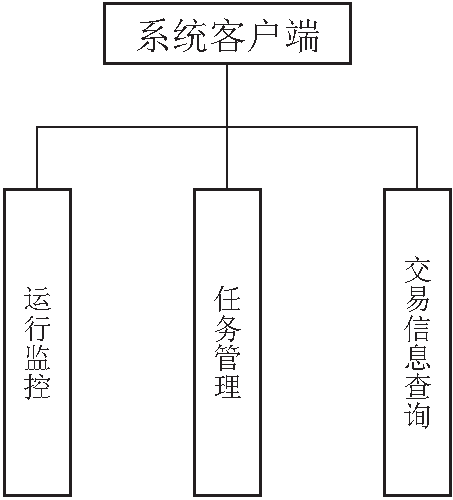
\includegraphics[width=\textwidth]{images/2.1-client.ps}
    \caption{客户端操作呈现功能树}
    \label{fig:client}
  \end{subfigure}
}

\subsection{系统可行性分析}
\subsubsection{经济可行性}
通过采用与加密货币思路类似的分布式部署和轻量化溯源(指线性时间复杂度的溯源方案),使得区块链监控与溯源系统不需要超高性能的计算机,使用三台监控节点即可对数千乃至上万的加密货币入口节点形成有效监控\cite{biryukov2014deanonymisation},而对于国家机器而言,部署数百台乃至数千台监控节点对主要加密货币进行监控,并通过对链上实时发生的交易进行追踪和去匿名化工作实施对加密货币交易监管,对数以亿计的洗钱、赌博资金流向监控与拦截能起到有效的杠杆支撑作用。
\subsubsection{社会可行性}
加密货币广受犯罪分子的青睐,被频繁用于洗钱、赌博与非法黑市交易,这对国家的网络安全发展构成了严重的危害。区块链公有链系统去中心、自治化、强匿名等特性导致政府和机构无法对公有链系统进行有效的监管。通过构建监控溯源系统对加密货币的交易进行监控是符合政府法治维持社会安定的一贯政策的。而通过模仿加密货币客户端的行为,在一台计算机上与数千乃至上万个加密货币服务端进行连接并不会显著增加加密货币通信网络的压力,在这种情况下对比整个加密货币网络终端节点的数目,监控系统的影响是微乎其微的,故而并不会对正常使用加密货币的用户造成影响。

\subsection{开发工具分析及选择}
\subsubsection{Golang}
Go 是一种在语法上类似于 C,但具有内存安全、垃圾收集、结构类型和 CSP\cite{roscoe1998theory} 风格并发性的静态类型编译编程语言。其开发人员旨在摒弃其它编程语言弊端的同时,仍从其他语言保留了实用的特性:
\begin{itemize}
  \item 具有类似C语言的静态类型和运行效率
  \item 具有类似Python和Javascript这类脚本语言的易读性和易用性
  \item 具有高性能的网络处理和多线程处理能力
\end{itemize}

Go语言通过一种名为 goroutine的轻量级进程实现并发处理,goroutine的底层是通过协程来实现的。协程和线程一样共享堆,不共享栈,调度由不经由操作系统控制,故而协程能够避免无意义的调度;同时执行协程只需要极少的栈内存(大概是4\textasciitilde 5KB),而默认情况下线程栈的大小为1MB,因此在需要大量创建和切换上下文的语义下使用协程可以大幅提高性能。在Go语言中,以 go 关键字为前缀的函数调用会在新的 goroutine 中启动一个函数,goroutine就是一段代码,一个函数入口,以及在堆上为其分配的一个堆栈。所以在运行时创建的成本非常廉价,可以很轻松的创建上万个无需操作系统调度执行的goroutine。

同时,Go语言有着非常丰富的框架和工具库,相当一部分互联网使用Go语言承担其后端开发的同时给Go社区回馈了相当数量的开源项目,故使用Go语言开发高性能网络通信程序可以专注于处理业务逻辑而不必花大量精力去处理线程同步和网络socket通信,提升开发效率。
\subsubsection{RPC与kitex框架}
在分布式计算中,远程过程调用 (Remote Process Call, RPC) 是指计算机程序使子程序在不同的地址空间(通常在共享网络上的另一台计算机上)执行时,其编码就像普通的本地过程调用,而无需程序员显式编码远程交互的细节。也就是说,无论子程序是执行程序的本地程序还是远程程序,程序员都编写基本相同的代码。RPC是一种采用服务器-客户端(Client/Server)模式的系统,通过编写接口描述语言(Interface Description Language, IDL)以及RPC框架,程序员可以迅速的将一个过程的结果以原样形式发送给不在一台计算机上的客户端,极大提升开发的效率。

一次典型的RPC调用如\rfig{tech:rpc}所示,首先服务消费方(client)调用以本地调用方式调用服务;客户端存根(client stub)接收到调用后负责将方法、参数等组装成能够进行网络传输的消息体;client stub找到服务地址,并将消息发送到服务端;服务端存根(server stub)收到消息后进行解码;server stub根据解码结果调用本地的服务;本地服务执行并将结果返回给server stub;server stub将返回结果打包成消息并发送至消费方;client stub接收到消息,并进行解码;服务消费方得到最终结果。

\xfig{tech:rpc}{典型的RPC调用流程}{
  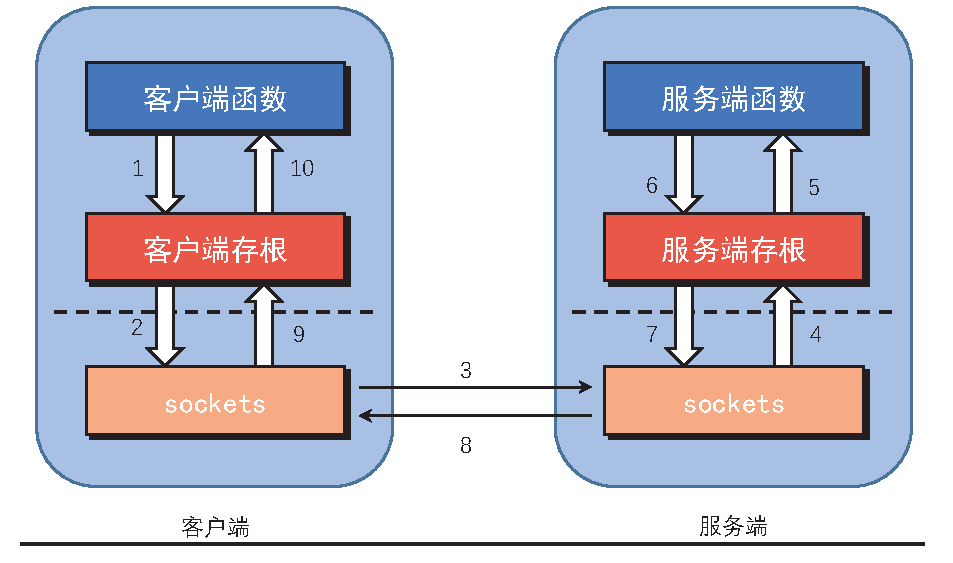
\includegraphics[width=\textwidth]{images/2.3-rpc.ps}
}

Kitex 曾是字节跳动内部的 Golang 微服务 RPC 框架,在2021年作为一个开源项目被发布到Github上,当前\footnote{指2022年5月。}已有4000个星标,是一个已经广泛应用的RPC服务框架,具有高性能、强可扩展的特点,支持多消息协议、多传输协议、多种消息类型,支持服务发现、监控、链路跟踪、自定义访问控制等治理特性,Kitex 内置代码生成工具,可支持生成 Thrift、Protobuf 以及脚手架代码,是分布式程序交互的理想选择对象,是实现监控节点向区块链公有链溯源监控系统获取任务和汇报监控消息的理想选择。
\subsubsection{WPF}

Windows Presentation Foundation (WPF) 是一个用于在基于 Windows 的应用程序中呈现用户界面的免费开源图形子系统。WPF提供了基于Direct3D的支持数据绑定、媒体服务、控件与数据模板、动画等特性的高性能用户界面支持。基于WPF的数据绑定特性,衍生出了名为MVVM(Model–View–ViewModel)的软件架构模式(\rfig{tech:mvvm})启示了当下流行的Vue.js、React.js等B/S(Browser/Server,浏览器/服务器架构)模式用户界面开发框架。MVVM有助于将图形用户界面的开发与业务逻辑或后端逻辑(数据模型)的开发分离开来:视图模型通过数据绑定负责从模型中暴露数据对象,并接受来自视图的事件更新。系统使用WPF开发用户界面可以使得界面代码、绑定代码、事件响应逻辑和后端处理逻辑可以轻松解耦合,极大提升开发的效率的同时降低开发难度和错误率。

\xfig{tech:mvvm}{MVVM模型概念}{
  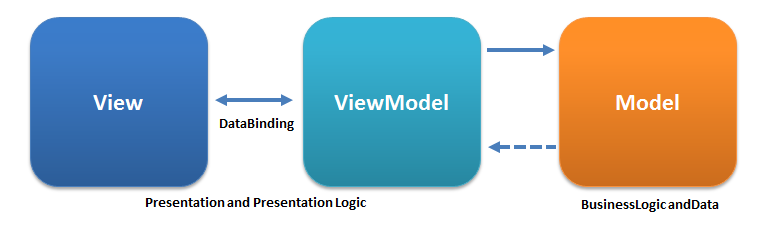
\includegraphics[width=\textwidth]{images/2.3-mvvm.png}
}
\subsection{关键技术分析}\label{sec:technique}
监控嗅探功能需要能够从获取到的带有时序的交易泛洪消息推测出交易消息的始发节点,故而需要采用消息随机传播源估计算法来找出可能的源节点,下面将简述名为首时间戳的估计器(\S \ref{fte})和名为报告中心的估计器(\S \ref{rce})。其中会将加密货币节点的对等网络建模为图$G(V,E)$,其中$V$是所有服务器节点的集合,$E$是它们之间的边或连接的集合;嗅探节点向每个服务器建立有固定数量$\theta$的连接($\theta\geq 1$)。

同时多节点系统时间不同步可能导致估计不准确,所以本文将在\S \ref{timesync}中将简述一种时间同步的方法。
\subsubsection{首时间戳估计器}\label{fte}
记监控嗅探节点首次从节点$v\in V$观测到消息的时间戳为$\tau_v$,记$\tau=(\tau_v )_{v\in V}$是所有观测到的首时间戳的集合。首时间戳估计器的识别源节点给出的候选节点即为$\text{M}_{\text{FT}} = \arg \min_{t\in V_t} \tau_v $,它输出在估计时间$t$之前向嗅探节点报告消息的第一个节点。这个方法是简单而自然的——即认为第一个向嗅探服务器报告的节点即为源节点。Fanti等人证明了\cite{fanti2017anonymity,fanti2017deanonymization}采用首时间戳估计器对现行泛洪协议的准确度不低于:
\begin{equation}
\frac{\theta}{d-2} \log{\frac{d+\theta - 2}{\theta}}\overset{\mathrm{bitcoin}}{=}\frac{\theta}{6} \log{\frac{6+\theta}{\theta}}
\end{equation}
\subsubsection{报告中心估计器}\label{rce}
假设已被报告消息的加密货币网络子树$G_t$的根节点为$w$;记$T_v^w$为子树$G_t$中包含节点$v$及其所有关于根节点$w$的孩子的子树。对于随机变量$Y_v (t)$,在$t$时刻,若节点$v\in V$已经向对手报告,则其值为1,否则为0。令$Y_{T_v^w} (t)=\sum\limits_{u\in T_v^w} Y_u (t)$来表示在$t$时刻子树$T_v^w$中已经向监控节点通知交易的节点个数;令$Y(t)=\sum\limits_{v\in V_t} Y_v (t)$来表示在$t$时刻子树$G_t$中已经向监控节点通知交易的节点个数。类似地,用$N_{T_v^w} (t)$来表示在$t$时刻子树$T_v^w$中已经获知交易消息的加密货币节点个数(因此$N_{T_v^w} (t)\geq Y_{T_v^w}(t)$),用$Y(t)$来表示在$t$时刻已经获知交易消息的节点个数($N(t)\geq Y(t)$)。对于每个候选源$v$,考虑它由集合$N(v)$组成的$d$个邻居。在$t$时刻节点$v$的报告中心(记作$R_v (t)$)定义如\reqn{rce}:
\begin{equation}
  R_v(t)=\left\{
    \begin{array}{ll}
      1 & \text{if}\  \max_{u\in N(v)} Y_{T_u^v}(t)<\frac{Y(t)}{2}  \\
      0 & \text{otherwise.}
    \end{array}
  \right. \label{eqn:rce}
\end{equation}

也就是说,当每个相邻子树的报告节点少于$Y(t)/2$(整个已得到消息的子树节点数目的一半)时,节点的报告中心度为1。如果节点的报告中心度为1,则该节点为报告中心。报告中心估计器输出从所有报告中心均匀选择的一个节点$v$,作为其估计的传播源。\rfig{rce}举出了一个$Y(t)=5$,$N(t)=7$的例子,其中$R_{v^*}(t)=1$,$R_{w}(t)=0$,故图中$v^*$是一个报告中心。Fanti等人证明了\cite{fanti2017anonymity,fanti2017deanonymization}采用报告中心估计器对现有加密货币交易信息源估计有着较好的结果。
\xfig{rce}{报告中心估计的一次子树节点状态}{
  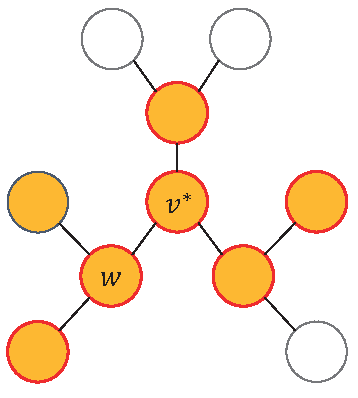
\includegraphics[width=0.2\textwidth]{images/2.4-rce.ps}
}


\subsubsection{时间同步协议}\label{timesync}
采取多个嗅探节点对比特币网络进行嗅探,若嗅探节点的时间不同步,在不同节点处对同一交易记录的时间戳可能存在误差,在不同节点中便可能引起首时间戳估计的错误,在同一组(连接到相同的加密货币局部节点网络)的嗅探节点间,需要完成时间同步。网络时间协议\cite{mills2010network}(Network Time Protocol,NTP)是在数据网络潜伏时间可变的计算机系统之间通过分组交换进行时钟同步的一个网络协议,位于OSI模型的应用层。
典型的NTP客户端将定期轮询不同网络上的三个或更多服务器。为同步其时钟,客户端必须计算其时间偏移量和来回通信延迟。时间偏移“$\theta$”定义为:

\begin{equation}
  \theta=\frac{(t_1-t_0 )+(t_2-t_3)}{2}
\end{equation}

往返延迟“$\delta$”为:
\begin{equation}
  \delta=(t_3-t_0 )-(t_2-t_1)
\end{equation}

其中:$t_0$是请求数据包传输的客户端时间戳,$t_1$是请求数据包回复的服务器时间戳,$t_2$是响应数据包传输的服务器时间戳,$t_3$是响应数据包回复的客户端时间戳。

通过此协议,监控嗅探节点在向系统后端报告监控得到的结论时可以采用系统后端的时间,消除系统各节点时间不统一导致结论出现冲突的问题。

\subsection{本章小结}

本章首先对开发一个区块链公有链交易监控与溯源系统产生的需求进行了分析,然后对系统开发的可行性进行了分析;通过需求本章论证了选取Golang语言、kitex框架以及WPF技术开发系统的原因;最后本章对开发系统中需要使用的关键技术(溯源估计方法和时间同步方法)进行了简要分析和论述,为设计和实现该系统打下基础。

\newpage
\section{系统设计}

前面论述了设计与实现一个区块链公有链交易监控与溯源系统的需求,并分析了这些需求所对应需要的技术实现手段和理论基础。本章将自顶向下设计一个可以完成前述需求的交易监控溯源系统(下称“Argos”系统),并对系统功能模块进行划分,为后续实现Argos系统提供脚手架。
\subsection{系统总体设计}

\subsubsection{系统网络拓扑}
为应对复杂多变的网络环境和监控任务情况,Argos系统网络采用分布式技术实现,并采用RPC和HTTP进行节点间的相互通信,为了实现数据有效和安全的存储,选取MySQL进行数据存储。通过使用netpoll\footnote{Netpoll 是由字节跳动开发的高性能 NIO(Non-blocking I/O) 网络库,专注于 RPC 场景。\url{https://github.com/cloudwego/netpoll}。}高性能网络通讯库,在零拷贝\cite{stancevic2003zero}的情况下读取加密货币网络通信数据,使得数据吞吐量大大提高,从而使得一个监控节点可以承载更多的加密货币节点通讯需求。系统的网络拓扑在\rfig{system:topology}中描述。


\xfig{system:topology}{Argos系统网络拓扑}{
  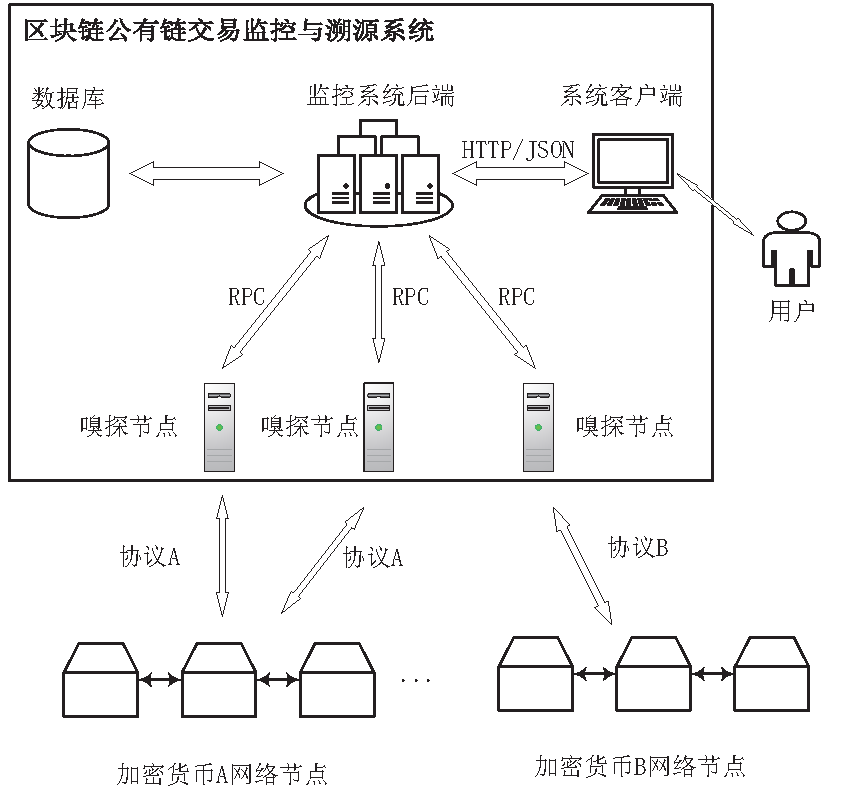
\includegraphics[width=0.65\textwidth]{images/3.1-topology.ps}
}


监控嗅探节点通过thrift\footnote{Thrift是一种被用来定义和创建跨语言服务的接口描述语言和二进制通讯协议。\url{https://github.com/apache/thrift}。}定义的IDL经Kitex框架与Argos系统后端通讯。Argos系统客户端通过Argos系统后端提供的HTTP/JSON接口查询获取得到的去匿名化交易监控记录。

\subsubsection{系统软件架构}

Argos监控溯源系统是多节点的C/S架构程序,\rfig{system:strcuture}给出了Argos系统的软件架构。Argos系统核心主要分为Argos客户端、后端和嗅探节点端三大模块,同时为了与具体的加密货币节点进行通信获取信息,需要根据具体加密货币的通信协议约定,实现托管式的加密货币端(下称Peer)交互模块。

\xfig{system:strcuture}{Argos系统软件架构(图中略去了嗅探模块与Peer交互模块的关系)}{
  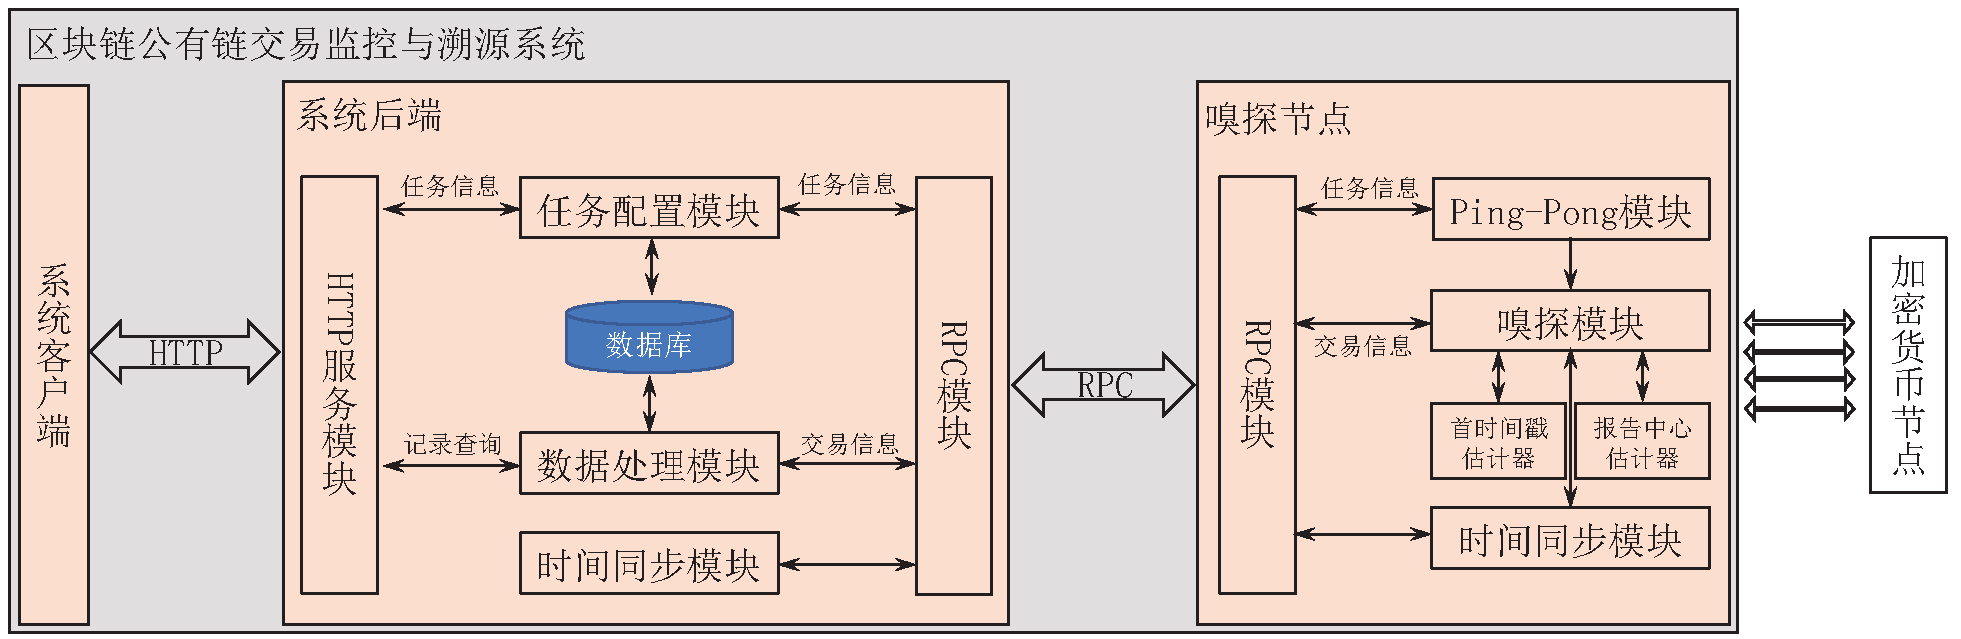
\includegraphics[width=\textwidth]{images/3.2-structure.ps}
}

下面对这几个模块进行简要介绍:

\textbf{Argos客户端模块}\ 提供可视化的操作界面,简述系统运行情况,提供编辑节点任务的配置功能以及按不同方式查询系统获取的去匿名化的交易信息的功能。

\textbf{Peer交互模块}\ 提供抽象化的一个被系统需要的加密货币的Peer连接的功能。

\textbf{Argos后端模块}\ 是系统核心的中央处理模块,用于沟通嗅探模块和客户端,通过连接到数据库提供任务和信息存储功能。

\textbf{Argos监控嗅探模块}\ 是系统中最小的加密货币子网交易信息处理单元,得出子网中交易信息的可能源头进行上报。

\subsubsection{开发环境}
整个系统不同的模块有不同的部署场景,为了符合一般应用中后端常在linux环境运行的状态,嗅探节点和系统后端在一运行Manjaro Linux的虚拟机中开发,使用的集成开发环境为Visual Studio Code。对于最终用户,一般使用Windows桌面操作系统,故客户端选择在宿主机上开发,宿主机运行Windows 10操作系统,使用的集成开发环境为Visual Studio 2022 Community。整个系统均在一台搭载AMD Ryzen 5800H 8C16T的x86笔记本上开发,配置有32GB运行内存。
\subsection{功能模块设计}
\subsubsection{Peer交互模块}
Peer交互模块是Argos系统中直接与指定的加密货币节点有信息交互的节点,托管所有的socket通信。Peer交互模块提供一种从加密货币通信协议到被Argos系统嗅探模块所需的抽象,使得系统其他部分可以在不与具体加密货币通信协议与处理耦合的情况下,通过调用由Peer抽象出的建立连接、网络拓扑获取和交易信息获取功能获取系统完成去匿名化的功能,而Peer交互模块和其下挂载的具体加密货币通信协议实现负责真正的通信。

\xfig{module:peer}{Peer交互模块设计}{
  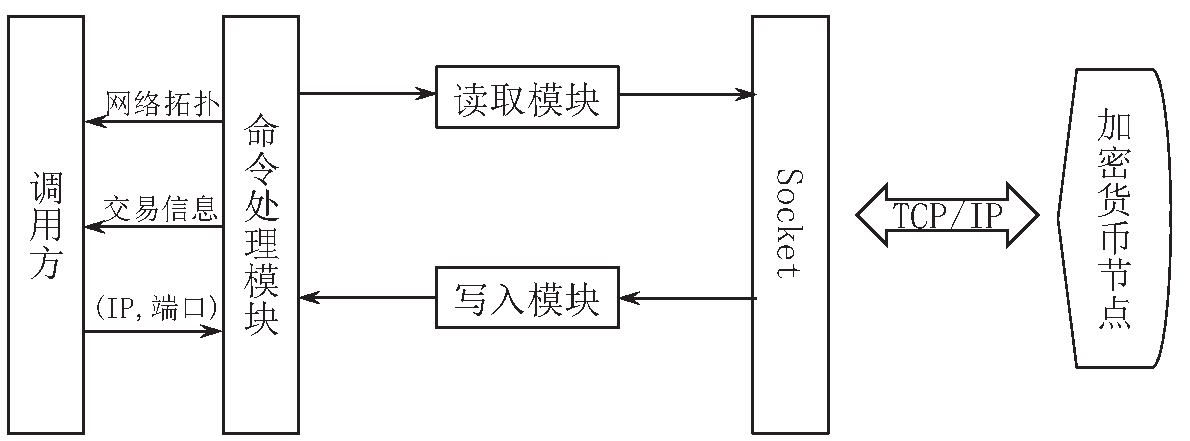
\includegraphics[width=0.8\textwidth]{images/3.3-peer.ps}
}

通过Peer交互模块的抽象,调用方只需使用目标地址(IP,端口)的元组,即可创建一个可以产出必要信息的Peer连接。
\subsubsection{Argos监控嗅探模块}
监控嗅探模块根据Argos系统后端下发的任务指令,从由加密货币协议提前约定的节点查询DNS查询入口节点,从DNS解析获取的IP和加密货币约定的通信端口启动数个Peer交互模块实例作为接入的加密货币边缘网络。随后这数个Peer交互模块实例连接到目标节点后,会发送一系列握手和通信包,在获取到邻接节点信息后回调监控嗅探模块的邻节点回调接口;监控嗅探模块根据获取的邻居节点信息创建更多的Peer交互模块实例,逐步连接到加密货币网络的一个子网。在连接到足够数量的节点后开始对获取到的交易信息持续运行\S \ref{sec:technique}中给出的估计算法,上报到系统后端进行分析和存储。
\begin{figure}[H]
  \centering
  \begin{minipage}{0.48\textwidth}
    \centering
    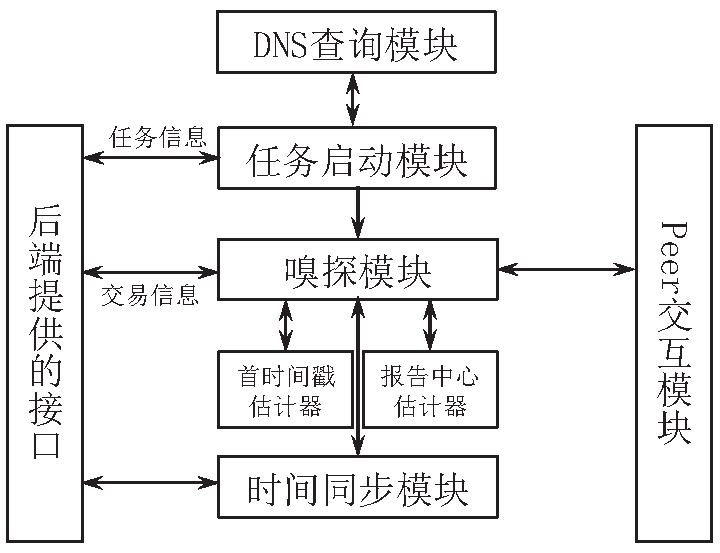
\includegraphics[width=\linewidth]{images/3.3-sniffer.ps}
    \caption{Argos监控嗅探模块设计}\label{fig:module:sniffer}
  \end{minipage}\hfill
  \begin{minipage}{0.48\textwidth}
    \centering
    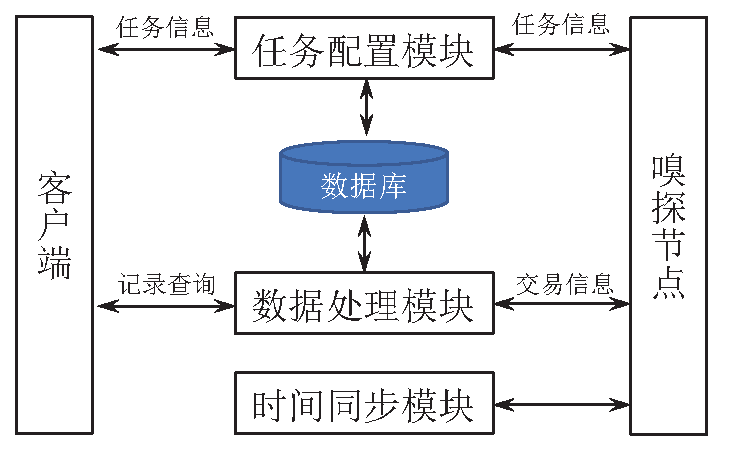
\includegraphics[width=\linewidth]{images/3.3-master.ps}
    \caption{Argos后端模块设计}\label{fig:module:master}
  \end{minipage}
\end{figure}
为了使得上报到Argos系统后端的数据在不同监控嗅探模块间不会由于不同节点操作系统时间不统一的问题产生歧义,监控嗅探模块需要在运行监控任务的同时周期性(Argos系统设计为10s)的向系统后端发送时间同步请求,通过多个时间戳消弭时间同步请求在经TCP(Transmission Control Protocol,传输控制协议)传输的延迟,从而获得Argos系统后端与当前节点时间戳差,利用差值在上报信息时对时间戳进行补正,解决时间同步问题。
\subsubsection{Argos后端模块}
Argos系统后端模块连接到MySQL数据库,根据客户端发来的配置更新任务列表,并下发到嗅探模块;根据嗅探模块上报的去匿名化交易信息向数据库中保存最佳结论,并向客户端根据时间、IP、交易等不同维度的选择在数据库中查询响应的信息;提供与嗅探模块进行时间同步的功能。


\subsubsection{Argos客户端模块}
Argos客户端模块展示系统运行情况,提供任务的配置和查询功能,同时提供最终去匿名化的加密货币交易信息查询功能,根据不同的需求情况,分为按时间查询加密货币的去匿名化状态、分IP和交易视角查询加密货币去匿名化信息提交历史,提供一个完整全面的加密货币交易信息去匿名化用户界面,其页面划分如\rfig{module:client}所示。

\xfig{module:client}{Argos客户端页面设计}{
  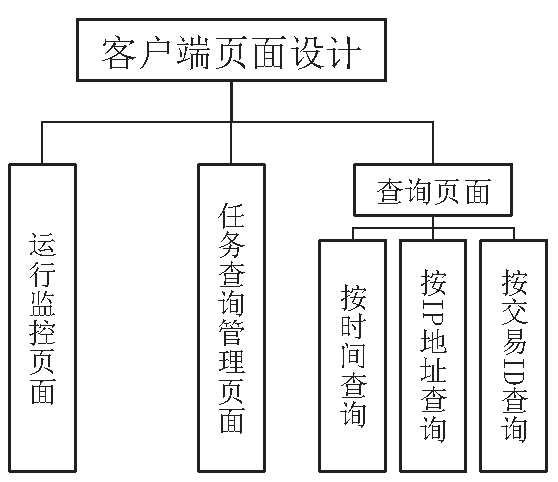
\includegraphics[width=0.5\textwidth]{images/3.3-client.ps}
}

\subsection{本章小结}
本章自顶向下从整体网络拓扑到各个模块子功能划分,设计了一个可以完成\S \ref{sec:demands}论述需求的监控溯源系统,详细说明了各个模块互相交互的信息传递,根据需求给出了各个功能的设计细节,为下面实现Argos系统提供设计上的总体指导。
\newpage


\section{系统实现}
在前面两章中,完成了对Argos系统的方案论证和总体设计,这一章将会讨论系统的具体实现。

\subsection{Peer交互模块实现}\label{sec:peer}
Peer交互模块是抽象封装了Argos系统全部所需的加密货币的通信协议的模块,本系统包含了Peer交互模块的接口和一套实现该接口的比特币Peer交互模块,模块实现了比特币的通信协议,通过在网络数据流中识别特征魔数,通过通信子模块解析出比特币数据包,交由处理托管子模块进行处理和回应,将本系统需要的邻节点数据和交易消息留存回调上报。
\subsubsection{比特币协议}
本文所述比特币协议是指比特币官方参考客户端\footnote{比特币官方客户端参考指bitcoind,是比特币开源项目Bitcoin Core的一部分。\url{https://github.com/bitcoin/bitcoin/。}}所使用的RPC通信协议。该协议的所有消息均有着相同的数据结构,其数据包的数据结构如下:
\begin{minted}[linenos=true]{c}
typedef struct {
    uint32_t magic;         // 识别消息头的魔数,同时决定网络类型。
    char     command[12];   // 命令类型
    uint32_t length;        // 载荷长度
    uint32_t checksum;      // 载荷校验
    char     payload[0];    // 变长数组,承载载荷
} Message;
\end{minted}


所有的消息前均包含一24字节长的消息头:magic字段用于在无序socket流中标记一个数据包的起始点,同时存储有网络注册信息;command字段标识当前数据包载荷命令的类型,\rtbl{peer:cmd}记录了被比特币协议实现使用的命令及命令的含义与作用;length和checksum字段分别标识载荷的长度和校验码。

\begin{generaltab}{比特币协议实现用到的命令}{tbl:peer:cmd}
  \begin{tabular}{c|ccc}
    \toprule
    command & 用途  \\
    \midrule
    version & 标识有关程序版本和区块的信息。节点第一次连接时交换version信息。\\
    verack  & 响应版本消息发送,以确认节点愿意连接。 \\
    addr    & 列出节点邻节点 \\
    inv     & 通知区块和交易的发生,用于节点中继转发这些信息。\\
    tx      & 传递交易信息 \\
    \bottomrule
  \end{tabular}
\end{generaltab}

为应对实际网络连接中可能出现的信息流状态丢失的问题,比特币协议采用了magic数字用于标识有效信息包的起始状态,同时不同的比特币网络\footnote{比特币存在包括但不限于mainnet、testnet等的网络,不同网络间并不互通,mainnet为实际真实的用户网络,其他网络一般用于开发和功能测试。}共对应五种不同的magic代码(见\rtbl{peer:magic}),根据五种magic设计一个状态机即可完成识别和检测。
\begin{generaltab}{比特币magic码}{tbl:peer:magic}
  \begin{tabular}{c|ccccc}
    \toprule
    magic名/网络名    & 第一位 & 第二位 & 第三位 & 第四位 & 完整magic码\\
    \midrule
    main             & \texttt{0xF9} & \texttt{0xBE} & \texttt{0xB4} & \texttt{0xD9} & \texttt{0xD9B4BEF9}\\
    namecoin         & \texttt{0xF9} & \texttt{0xBE} & \texttt{0xB4} & \texttt{0xFE} & \texttt{0xFEB4BEF9}\\
    testnet/regtest  & \texttt{0xFA} & \texttt{0xBF} & \texttt{0xB5} & \texttt{0xDA} & \texttt{0xDAB5BFFA}\\
    testnet3         & \texttt{0x0B} & \texttt{0x11} & \texttt{0x09} & \texttt{0x07} & \texttt{0x0709110B}\\
    signet(default)  & \texttt{0x0A} & \texttt{0x03} & \texttt{0xCF} & \texttt{0x40} & \texttt{0x40CF030A}\\
    \bottomrule
  \end{tabular}
\end{generaltab}

\subsubsection{比特币Peer通信的工作流程}
比特币Peer采用netpoll进行TCP网络通信,流程图见\rfig{impl:peer},在模块被调用后启动两个协程进行工作:



\textbf{读取协程}\ 在判定连接套接字有效后启动一自动机识别\rtbl{peer:magic}中规定的起始码,识别后解析出命令名称、包长度和包校验,读取完整个包长度的数据后对数据包的校验码进行校验。随后根据不同命令解析出对应的数据包交给对应的处理(handle)函数。

\textbf{写入协程}\ 根据待写入的数据包通道(channel),不断从通道中获取已经待写入的数据包,按照数据包头要求封包完成后传入套接字。

\xfig{impl:peer}{比特币Peer流程图}{
  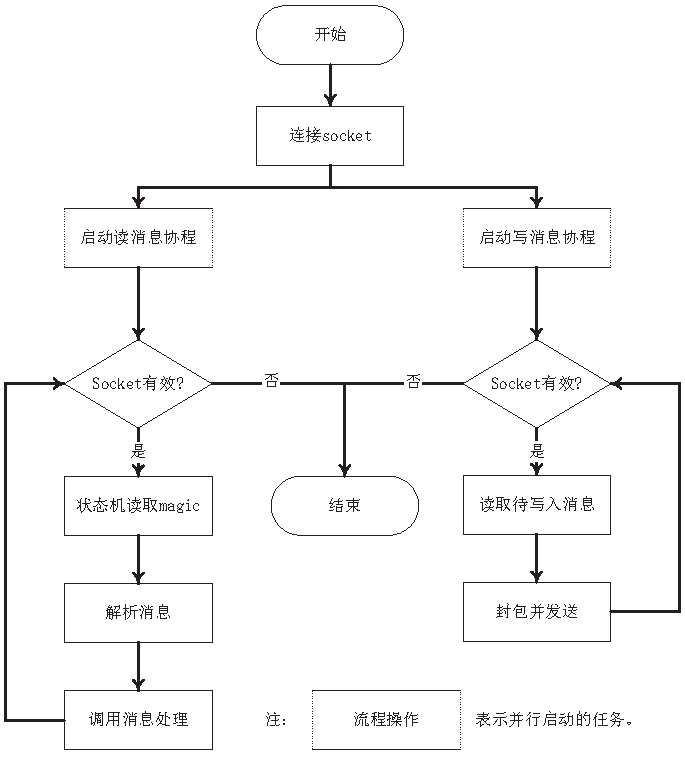
\includegraphics[width=0.9\textwidth]{images/4.1-peer.ps}
}

\subsubsection{比特币Peer的托管处理}
参考Satoshi开发的参考客户端的行为,比特币Peer连接从建立到托管的全流程如下:

(1)Peer交互模块根据给定的(IP,端口)元组建立TCP连接。

(2)Peer交互模块组织代表自身节点的version数据包通过TCP连接发送至远程节点。

(3)Peer交互模块收到来自远程节点的version数据包和verack数据包,在自身回应一个verack数据包后进入监听状态。

(4a)Peer交互模块收到来自远程节点的addr数据包,解析为Argos系统所接受的数据结构后调用嗅探模块提供的邻节点回调。

(4b)Peer交互模块收到来自远程节点的inv数据包,将标识为交易的项目解析为Argos系统所接受的数据结构后调用嗅探模块提供的交易回调。

(4c)Peer交互模块收到来自远程节点的其他数据包,有需要返回数据的根据比特币通信协议给出相应的响应,限于篇幅不一一介绍。

(5)网络波动或远程Peer主动断开,Peer交互模块退出。

下面以一名称为“inv”的命令的处理为例,介绍处理函数的实现。inv命令的数据结构如下:
\begin{minted}[linenos=true]{c}
typedef struct {
    struct {
        uint64_t val;
        char     data[0];
    } count;
    struct {
        uint32_t inventoryType;
        char     hash[32];
    } inventory[0];
} CmdInv;
\end{minted}

inv命令的用途是在端点间用于通知新的数据产生的一种泛洪消息。其中count字段标识inventory字段的长度,采用一种依据首位数字决定位数的数字压缩变长编码:首位若小于0xFD,编码数字为一个字节长;首位等于0xFD,编码数字为两个字节长;首位等于0xFE,编码数字为四个字节长;首位等于0xFF,编码数字为八个字节长。inventory字段为一前面count指定长度的列表,即为存放新的区块或交易的标识符的区域。inventory结构体中inventoryType标识当前inv命令通知的消息的类型,包括交易、新区块等。

故inv命令处理函数只需先根据数据结构从二进制数据中解析出inv命令结构,循环读取inventory数组,将标记为交易的哈希值上报监控嗅探模块即可。

\subsection{后端存储管理模块实现}
后端模块通过连接到MySQL数据库,根据客户端发来的配置更新任务列表,并下发到嗅探模块;根据嗅探模块上报的去匿名化交易信息向数据库中保存最佳结论,并向客户端根据时间、IP、交易等不同维度的选择在数据库中查询响应的信息;提供与嗅探模块进行时间同步的功能。其时序图如\rfig{impl:seq}。

\xfig{impl:seq}{Argos后端模块时序图}{
  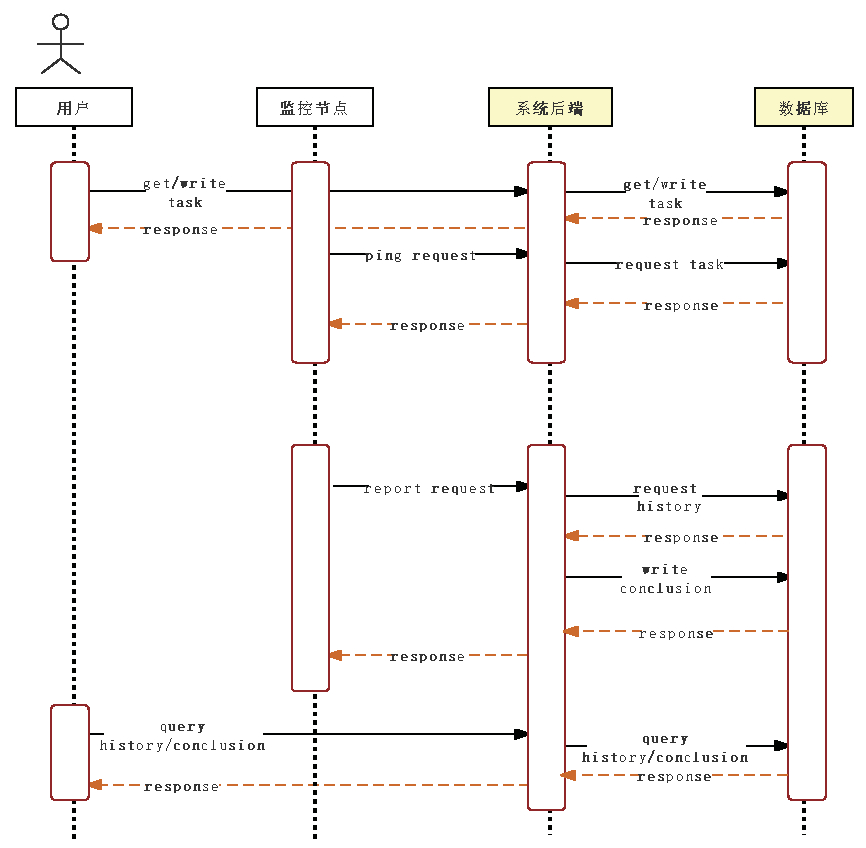
\includegraphics[width=\textwidth]{images/4.2-seq.ps}
}
\subsubsection{任务存储下发与时间同步}
为了使Argos系统成为不与某一加密货币强耦合,其在设计上是支持多协议的,故在分布式系统中对监控嗅探模块的任务分配与指令下发成为作为核心节点的后端存储模块的必要功能。建立如\rtbl{master:task}的数据表,其中id字段是自增的索引主键字段,prefix字段代表以此前缀的一组监控嗅探节点均下发以protocol为名称的加密货币协议进行监控。

\begin{generaltab}{任务表结构}{tbl:master:task}
  \begin{tabular}{c|ccccc}
    \toprule
    字段中文名          & 字段英文名 & 类型       & 可空      & 键值类型 & 其他属性\\
    \midrule
    任务编号           & id       & int         & NOT NULL & 主键 & auto\_{}increment\\
    任务组后端id前缀    & prefix   & char(255) & NOT NULL & 唯一 & /\\
    任务组协议         & protocol & char(255)  & NOT NULL & /   & /\\
    \bottomrule
  \end{tabular}
\end{generaltab}

任务存储下发与时间同步通过Argos后端存储管理模块的ping调用完成,其请求和响应的thrift数据结构如下:
\begin{minted}[linenos=true]{thrift}
  struct PingRequest {
      1: string identifier  // 监控嗅探节点实例唯一标识符
      2: i64 timestamp      // 请求时监控节点的时间戳
      3: optional i64 deltaTime // 当前时间差
  }
  struct PingResponse {
      // 响应状态,包括响应错误码和错误信息
      1: base.ResponseStatus status 
      // 下发的任务协议
      2: string   protocol  
      // 时间同步消息,包括嗅探节点发送,后端接受与发送三个时间戳
      3: TimeSync timeSync  
  }
\end{minted}

任务的存储下发与时间同步通过在收悉调用时立即缓存当时系统时间戳,随后根据唯一标识符中的连字符“-”分割获取前缀,连接数据库根据前缀查询对应的任务信息,获取到结果后将协议、收到请求中的时间戳、收悉请求时的时间戳和查询数据库完成后的时间戳存入响应pong消息中实现RPC调用约定。
\subsubsection{交易信息存储查询}
交易信息的存储分为两个部分:一方面,在收到各个监控嗅探节点上报的交易信息后数据需要立即入库,保存完整的历史溯源推测信息;另一方面,在得到同一交易的多个上报信息后,需要根据同一交易的不同节点根据局部网络给出的结论进行最佳选择\footnote{当前的选取策略采取和首时间戳估计法一样的策略,无论是首时间戳估计法得到的去匿名化交易信息还是通过报告中心估计法得到的去匿名化交易信息,在后端进行最终结论存储时再采取一次首时间戳估计作为最终结论。},以供结论化的展示。

根据上面的实现逻辑,需要建立两张表格,一张是作为Argos系统给出的最终估计的去匿名化交易信息结论表(conclusions表),另一张则是提供全局视角的去匿名化交易信息全数据表(records表),结构均如\rtbl{master:data}。

\begin{generaltab}{去匿名化交易信息表结构}{tbl:master:data}
  \begin{tabular}{c|ccccc}
    \toprule
    字段中文名          & 字段英文名 & 类型       & 可空      & 键值类型 & 其他属性\\
    \midrule
    记录id& id&	int	&NOT NULL &	主键	&	auto\_{}increment \\
    交易id& txid&	char(255)&	NOT NULL & /		&/\\
    时间戳& timestamp&	bigint&	NOT NULL &	/		&/\\
    源IP& source\_{}ip&	char(255)&	NOT NULL &		/		&/\\	
    监控节点标识符&sniffer&	char(255)&	NOT NULL &			/		&/\\
    交易协议& protocol & 	char(255)&	NOT NULL &			/		&/\\
    估计方法& protocol & 	char(255)&	NOT NULL &			/		&/\\
    \bottomrule
  \end{tabular}
\end{generaltab}

\subsection{监控嗅探模块实现}
实现一个区块链公有链交易监控与溯源系统最核心的目的是为了在有限的匿名化信息流中获取尽可能多的与交易相关的物理地址信息,对其进行去匿名化,监控嗅探模块即是实现这个核心功能的载体,下面将从Argos系统监控嗅探模块的核心工作流程和监视器两部分简述该模块的实现。
\subsubsection{监控嗅探模块核心工作流程}
去除运行状态等相关信息外,监控嗅探模块承载的数据可以抽象为下面一个数据结构(该数据结构是go语言风格结构定义):

\begin{minted}[linenos=true]{go}
type Sniffer struct {
    transactions chan argos.TransactionNotify
    newAddrs     chan net.TCPAddr

    network      *graph.Graph[addr, struct{}]
    notifies     map[[32]byte]map[addr]time.Time
    peers        map[addr]argos.Peer
}
\end{minted}

监控嗅探模块核心工作流程参可见\rfig{impl:sniffer}。

\xfig{impl:sniffer}{Argos后端嗅探模块核心工作流程图}{
  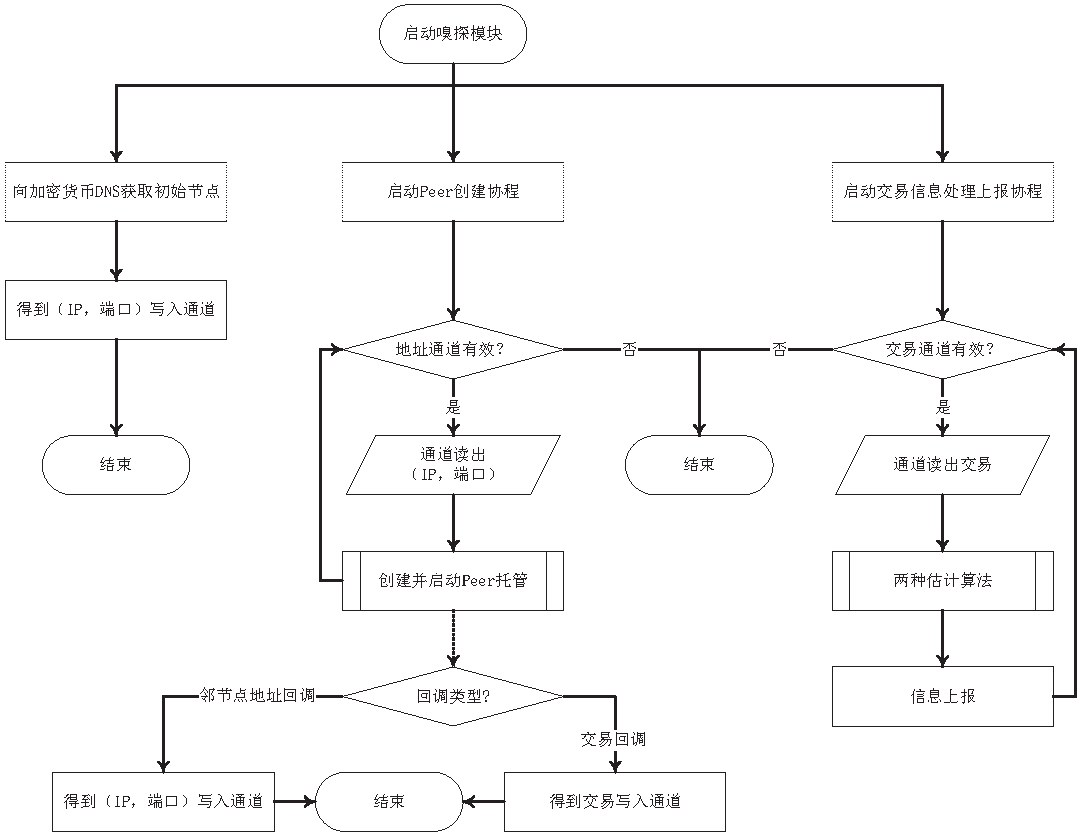
\includegraphics[width=0.98\textwidth]{images/4.3-sniffer.ps}
}

嗅探被监视器启动后,一方面向加密货币DNS请求,获取初始的种子节点,另一方面启动Peer创建托管和交易信息处理上报两个协程:

\textbf{Peer创建托管协程}\ 当通道有效且有数据时,不断从数据结构中newAddrs通道读取TCP远端地址,根据任务规定的加密货币协议启动\S \ref{sec:peer}实现的对应Peer,并设置关于邻节点和交易的回调函数(实际通过设计抽象的接口,将嗅探模块地址传入Peer中实现),在邻节点对应回调被调用时向newAddrs通道写入数据并将邻节点信息写入数据结构中network图中存储,在交易对应回调被调用时向transactions通道写入数据。

\textbf{交易信息处理上报协程}\ 当通道有效且有数据时,不断从数据结构中transactions通道读取交易通知,将通知时间写入数据结构中notifies这一分别以交易唯一标识符和交易信息发送地址为键值的映射中,以供核心根据\S \ref{sec:technique} 给出的两种估计方式实现的去匿名化估计算法使用。最后将产生传播源估计将信息上报系统后端处理。

\subsubsection{监控嗅探模块监视器}
监控嗅探模块需要定期检查当前节点任务列表以及与Argos系统后端同步时间,故需要实现一个监视器,用于检查监控嗅探模块(节点)的运行情况、检查任务是否改变以及同步时间。同步时间和任务可以通过后端存储模块提供的RPC Ping方法实现:监控嗅探模块每隔10秒向后端存储模块发送一个Ping请求,在返回后根据时间同步算法算出远程服务器与本机节点的时间差并保存,这个时间差在模块提交去匿名化的交易信息时被使用;检查时若发现当前节点任务改变,直接结束整个程序,重新开始运行。

Ping方法的PingResponse中的timeSync的thrift定义如下:
\begin{minted}[linenos=true]{thrift}
  struct TimeSync {
      1: i64 sendTimestamp
      2: i64 recvTimestamp
      3: i64 respTimestamp
  }
\end{minted}

故根据\S \ref{timesync}所述时间同步协议,补充监视器收悉响应的时间戳finalTimestamp,时间差$\theta$ 计算方式如\reqn{ts}所示。
\begin{equation}
  \theta=\frac{(\texttt{recvTimestamp}-\texttt{sendTimestamp} )+(\texttt{respTimestamp}-\texttt{finalTimestamp})}{2}\label{eqn:ts}
\end{equation}
\subsection{客户端模块实现}
Argos系统客户端采用WPF框架,使用MVVM架构实现,其页面结构如下:

-App.xaml: 程序资源配置文件  

-MainWindow.xaml: 主窗体页面

\qquad -QueryByAddressPage.xaml: 按IP地址查询页面

\qquad -QueryByTimePage.xaml: 按时间查询页面

\qquad -QueryByTransactionPage.xaml: 按交易查询页面

\qquad -StatusPage.xaml: 状态查看页面

\qquad -TaskConfiguewPage.xaml: 任务配置页面

主窗体采用NavigationView完成导航,将五种子页面嵌入到主窗体的Frame中。下面详细介绍主窗体导航实现。

主窗体的导航依据MVVM架构分为主窗体视图和主窗体视图模型两部分实现,两部分的交互逻辑见\rfig{impl:navigation}。

\xfig{impl:navigation}{Argos客户端主窗体视图模型交互逻辑}{
  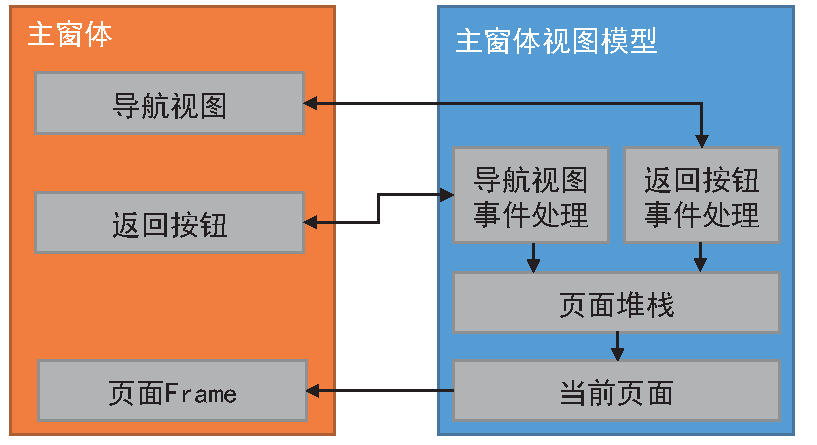
\includegraphics[width=0.9\textwidth]{images/4.4-navigation.ps}
}

其中,在视图中定义有包括两级导航菜单、回退按钮和页面的Frame,最终设计视图效果见\rfig{impl:navigation_result}。图中左侧即为导航菜单,在视图模型中设置有处理导航菜单选中项目和回退按钮受击的事件响应,收到事件发起后,这些事件响应程序将调整页面栈(使用一个栈结构将当前页面访问的历史记录保存了起来),随后调整Frame中对应的页面,完成导航的页面切换。

\xfig{impl:navigation_result}{Argos客户端主窗体视图呈现}{
  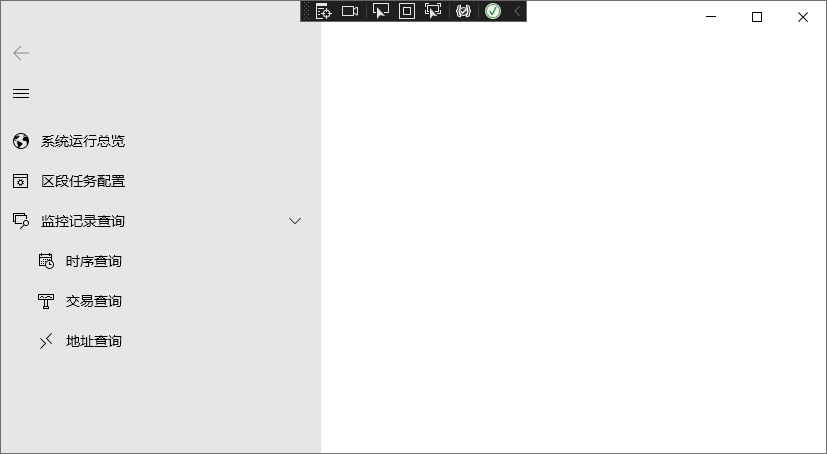
\includegraphics[width=0.9\textwidth]{images/4.4-navigation-result.png}
}
\subsection{设计中考虑的制约因素}
\textbf{社会因素考量}\ 在本文设计的区块链公有链监控与溯源系统中,采取了任务分配的设计,使系统嗅探模块的部署可以使用容器技术,拥有一定的自动运行能力,一定程度上避免了人工操作,降低了对人力成本的消耗,有利于社会生产力的提高。

\textbf{法律风险规避}\ 本系统的设计与实现均考虑了合法合规要求,开发的系统也是用于对可能存在的不法行为进行追踪;使用的开发语言、技术和功能库均采用开源技术,不存在专利侵权的可能;使用的需要动态或静态链接的开源项目不存在GPL协议的产品,不存在GPL传染的风险;所使用的集成开发环境、操作系统和撰写论文过程中使用的软件均为正版,不存在侵权问题。

\textbf{文化风险规避}\ 本系统的测试得到的数据在汇入本文前均经过了脱敏化;系统的代码、文档、测试方案中均不存在任何形式的暴力、威胁、反动、歧视、危害国家主权完整等不当言论的词汇和语句。

\subsection{成本估算}
软件开发成本估算主要指软件开发过程中所花费的工作量及相应的代价。不同与传统的工业产品,软件的成本不包括原材料和能源的消耗,主要是人的劳动的消耗。下面采用Putnam 模型对本系统开发成本进行估算。

Putnam 模型是1978年Putnam提出的,一种动态多变量模型。其核心模型见\reqn{putnam}。
\begin{equation}
  L = C_k * K^{\frac{1}{3}} * T_d^{\frac{4}{3}}\label{eqn:putnam}
\end{equation}

其中$L$是源代码行数(以LOC计),$K$是整个开发过程所花费的工作量(以人年计),$Td$是开发持续时间(以年计),$C_k$是技术状态常数,它反映“妨碍开发进展的限制”,取值因开发环境而异,见\rtbl{putnam}。

\begin{generaltab}{开发因素对$C_k$取值的影响}{tbl:putnam}
  \begin{tabular}{c|ccccc}
    \toprule
    $C_k$的典型值          & 开发环境 & 开发环境举例      \\
    \midrule
    2000&差&没有系统的开发方法,缺乏文档和复审\\
    8000&好&有合适的系统的开发方法,有充分的文档和复审\\
    11000&优&有自动的开发工具和技术\\
    \bottomrule
  \end{tabular}
\end{generaltab}

本系统开发时间从2022年2月初至2022年5月中,约3.5个月;开发使用Golang和成熟便捷的集成开发环境VS Code,并使用Git进行版本控制,开发环境定义为“好”,故$C_k$取8000,使用cloc软件统计,本系统后端共3118行Go语言代码,客户端共1132行布局XAML和行为C\#代码,记$L=4250$。计算得$K=20.72$。
\subsection{本章小结}

本章从第一小节的比特币交易Peer模块的实现开始,自底向上逐步实现了一个区块链公有链交易监控与溯源系统,并在接下来的三个小节中详细描述了该系统分层级的三个模块的具体实现;作为一个软件工程项目,在第五小节中本文讨论了设计中考虑的制约隐私,并在最后一小节估算了本项目的开发成本。

\newpage
\section{测试与分析}
前面已经对一个名为Argos的区块链公有链交易监控与溯源系统的实现做出了详细论证,作为一个软件工程项目,项目的测试与分析在设计与实现后是必不可少的部分,本文采用多种方式对Argos系统进行测试,以验证前文实现的正确性和可靠性。

\subsection{单元测试}
单元测试(Unit Testing),也称模块测试,是针对程序模块(软件设计的最小单位)来进行正确性检验的测试工作。单元测试的目标是隔离程序部件并证明这些单个部件是正确的。一个单元测试提供了代码片断需要满足的严密的书面规约。

Argos 系统开发时,对系统底层核心的通信模块等开发了完善的单元测试。下面介绍比特币通信模块的单元测试工作。

比特币的通信协议是一种自定义的RPC通信协议,其执行的远程调用函数命令在包头中给出,要实现比特币通信协议,首先就要实现对比特币通信协议中命令消息承载的载荷(Payload)进行二进制解析。这是实现比特币通信协议的最底层需求,也是对正确性要求最高的模块。在开发比特币通信模块时,其Peer实现中对于网络消息流的需求不是与其可靠传输连接套接字(TCP Socket)绑定的,通过简单的对象模拟(Object Mocking),将远程套接字的行为进行模拟,给出一定的二进制流,即可测试此部分实现的正确性。

二进制解析部分,设计有三种数据包的单元测试,分别为用于交换客户端信息的起始标识消息“version”、用于通知邻节点的泛洪消息“addr”和交易消息“tx”,这三个数据包的长度信息见\rtbl{test:data}。


\begin{generaltab}{二进制解析单元测试样例}{tbl:test:data}
  \begin{tabular}{c|ccccc}
    \toprule
    消息       & 消息字段数 & 长度       & 校验码\\
    \midrule
    version   & 8&	258	&\texttt{0xbecd93e2}  \\
    addr      & 1&	31&	\texttt{0x9b3852ed} \\
    tx        & 8&	101&	\texttt{0xec95d9c5}\\
    \bottomrule
  \end{tabular}
\end{generaltab}

同时由于二进制解析部分编写了几个工具函数,包括比特币协议常用的采取两次SHA-256的Hash函数、从某个数组中查询元素位置的Index函数和将Go语言的数组切片(Slice)转换为string的SliceToString函数,在比特币通信模块的单元测试中一并进行了测试。

单元测试的路径为protocol/bitcoin,运行测试与运行结果可见\rfig{test:unittest}。

\xfig{test:unittest}{单元测试结果}{
  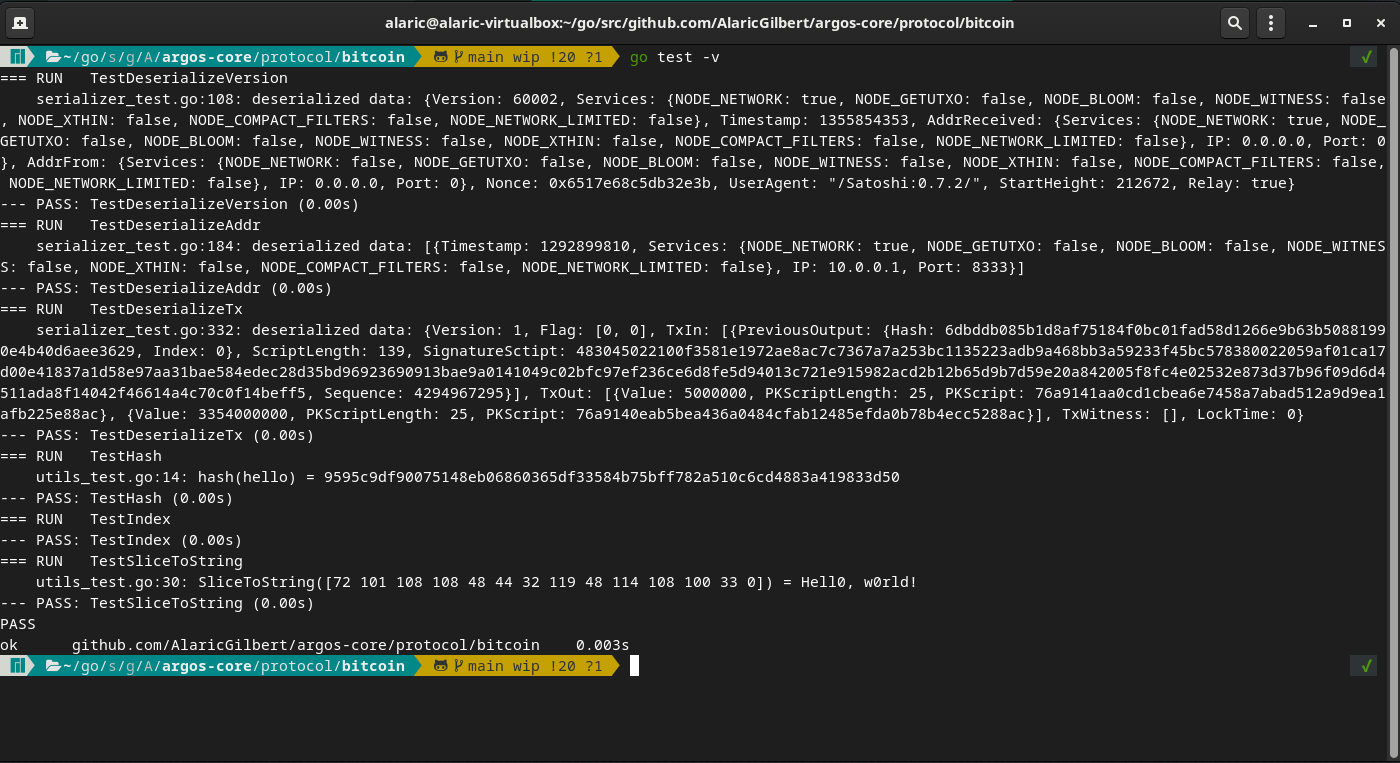
\includegraphics[width=0.9\textwidth]{images/5.1-unittest.png}
}

单元测试成功,说明此部分逻辑实现符合预期。

\subsection{后端接口测试}

后端提供的HTTP Web接口可以使用Hoppscotch工具进行测试,Hoppscotch是一种可以通过Web服务的方式构建API访问的工具,使用Node.js开发,采用简约的UI设计,能实时发送和获取响应值,其界面可见\rfig{test:hoppscotch}。

\xfig{test:hoppscotch}{Hoppscotch工具}{
  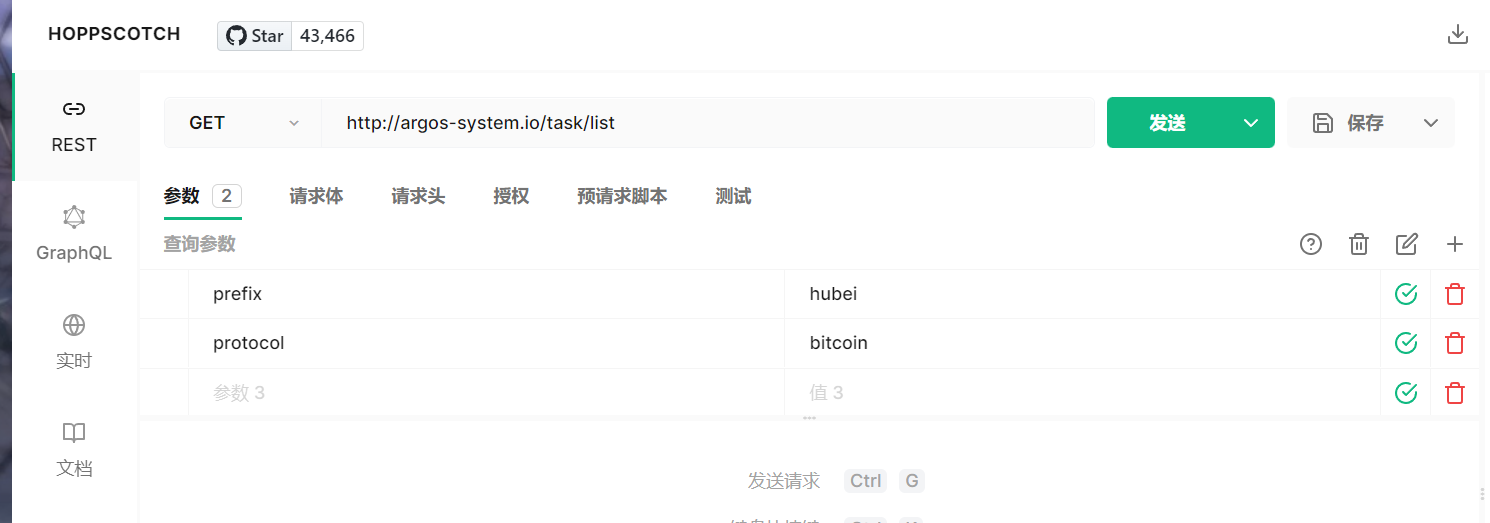
\includegraphics[width=0.9\textwidth]{images/5.2-hoppscotch.png}
}

在地址栏配置好要测试的API的URL,随后填写需要测试的查询参数,即可对HTTP接口进行测试。

下面以任务配置和获取接口为例,简述后端接口测试方案。任务配置和获取接口共计两组,路径分别为查询任务的/task/list和添加或修改任务的/task/write。首先对写入接口进行测试,编写如\rtbl{test:write_data}的测试集,其运行结果可见\rtbl{test:write_result}。

\begin{generaltab}{/task/write 接口测试集(反斜表示数据为空)}{tbl:test:write_data}
  \begin{tabular}{c|ccc}
    \toprule
    编号      & prefix & protocol       & 备注\\
    \midrule
    1        & hubei  &	bitcoin	& 为ID前缀为“hubei”的节点配置协议为“bitcoin” 的任务  \\
    2        & hunan  &	eth     & 为ID前缀为“hunan”的节点配置协议为“eth” 的任务 \\
    3        &   /    & test1   &	测试空前缀系统是否正常处理为报错\\
    4        & hk     & eth     &	为ID前缀为“hk”的节点配置协议为“eth” 的任务\\
    5        & hunan  & /       &	测试空任务是否正常处理为删除任务\\
    \bottomrule
  \end{tabular}
\end{generaltab}

\begin{generaltab}{/task/write 接口测试预期结果和实际结果}{tbl:test:write_result}
  \begin{tabular}{c|ccccc}
    \toprule
    编号      & 预期结果 & 实际结果       \\
    \midrule
    1        & 成功写入  &	接口返回代码“200”,代表写入成功	 \\
    2        & 成功写入  &	接口返回代码“200”,代表写入成功     \\
    3        & 参数错误  &  接口返回错误消息“prefix cannot be empty”,代表参数错误   \\
    4        & 成功写入  &  接口返回代码“200”,代表写入成功     \\
    5        & 成功删除  &  接口返回代码“200”,代表删除成功\\
    \bottomrule
  \end{tabular}
\end{generaltab}

在写入\rtbl{test:write_data}的测试集后,系统任务表应有两条数据:标识符前缀为“hubei”的节点配置协议“bitcoin”,标识符前缀为“hk”的节点配置协议“eth”,使用Hoppscotch工具进行对查询任务/task/list接口测试,获得如下的JSON响应:

\begin{minted}[linenos=true]{json}
{
    "code": 200,
    "tasks": [
        {
            "prefix": "hubei",
            "protocol": "bitcoin"
        },
        {
            "prefix": "hk",
            "protocol": "eth"
        }
    ]
}
\end{minted}

测试符合两条分别是为标识符前缀为“hubei”的节点配置协议“bitcoin”的信息和为标识符前缀为“hk”的节点配置协议“eth”的信息,说明此部分逻辑实现符合预期。
\subsection{嗅探节点测试}
嗅探节点所有主要运行流程中均有清晰日志呈现,在运行有后端模块的情况下,启动一个嗅探节点,即可测试嗅探节点功能是否运行正常。
\xfig{test:sniffer}{嗅探节点测试情况}{
  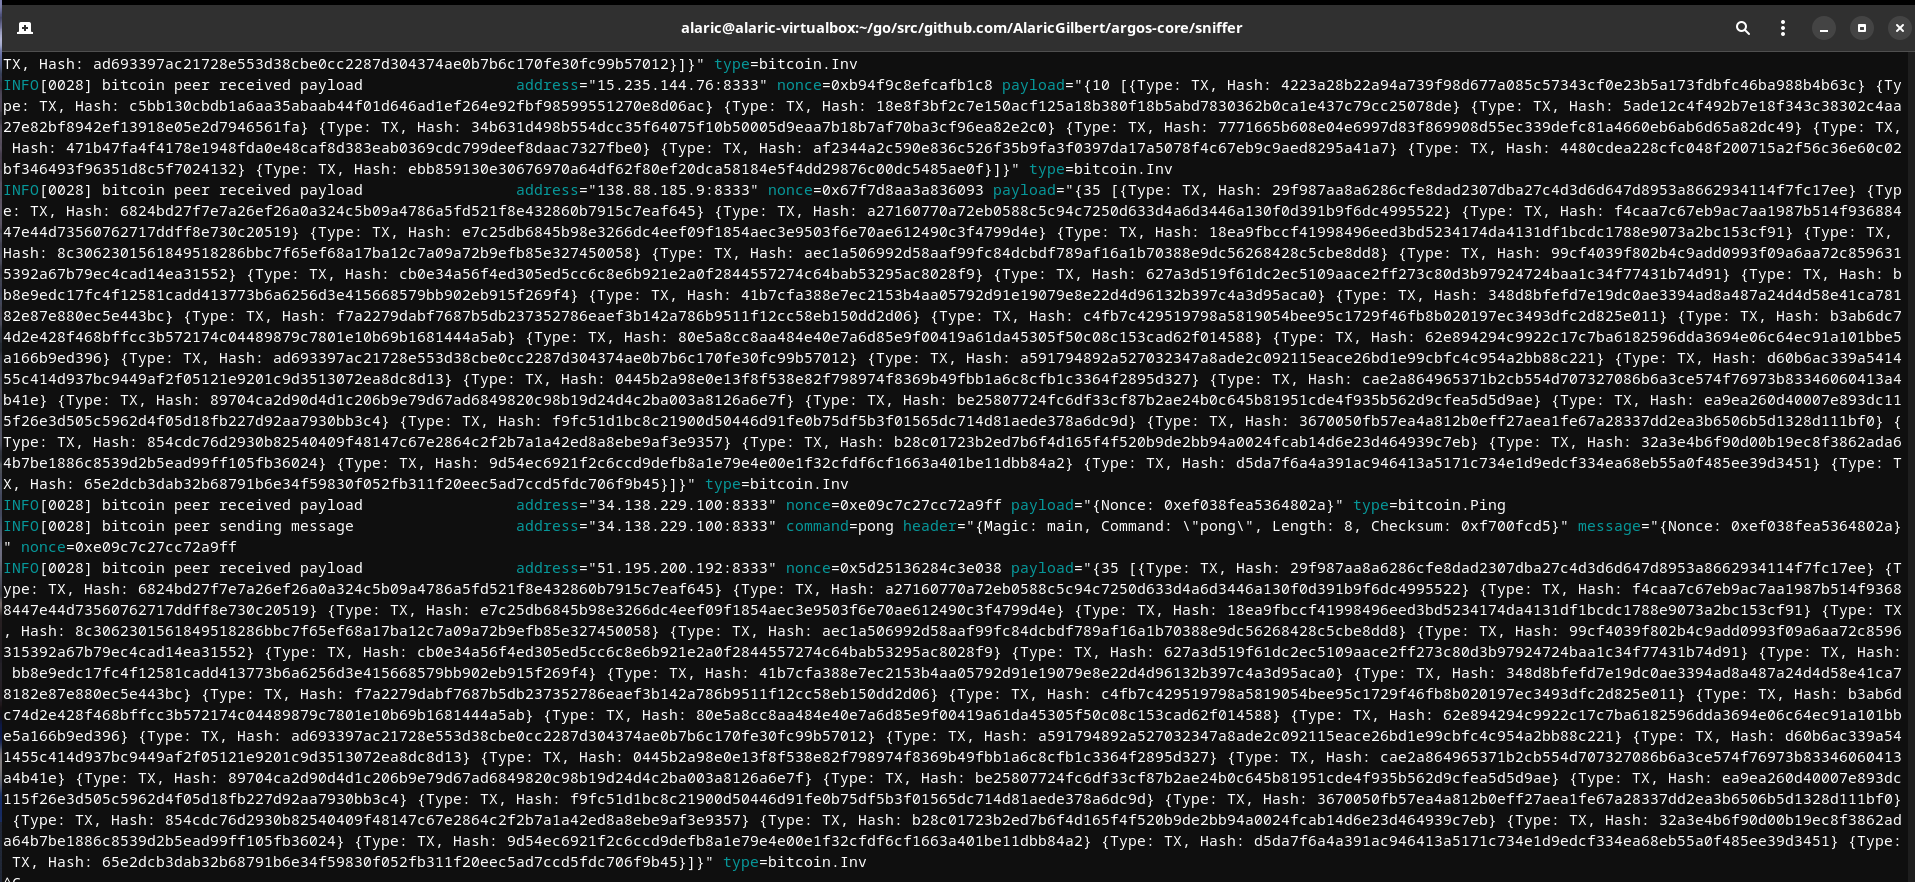
\includegraphics[width=\textwidth]{images/5.3-sniffer.png}
}
\xfig{test:master}{嗅探节点测试时后端节点情况}{
  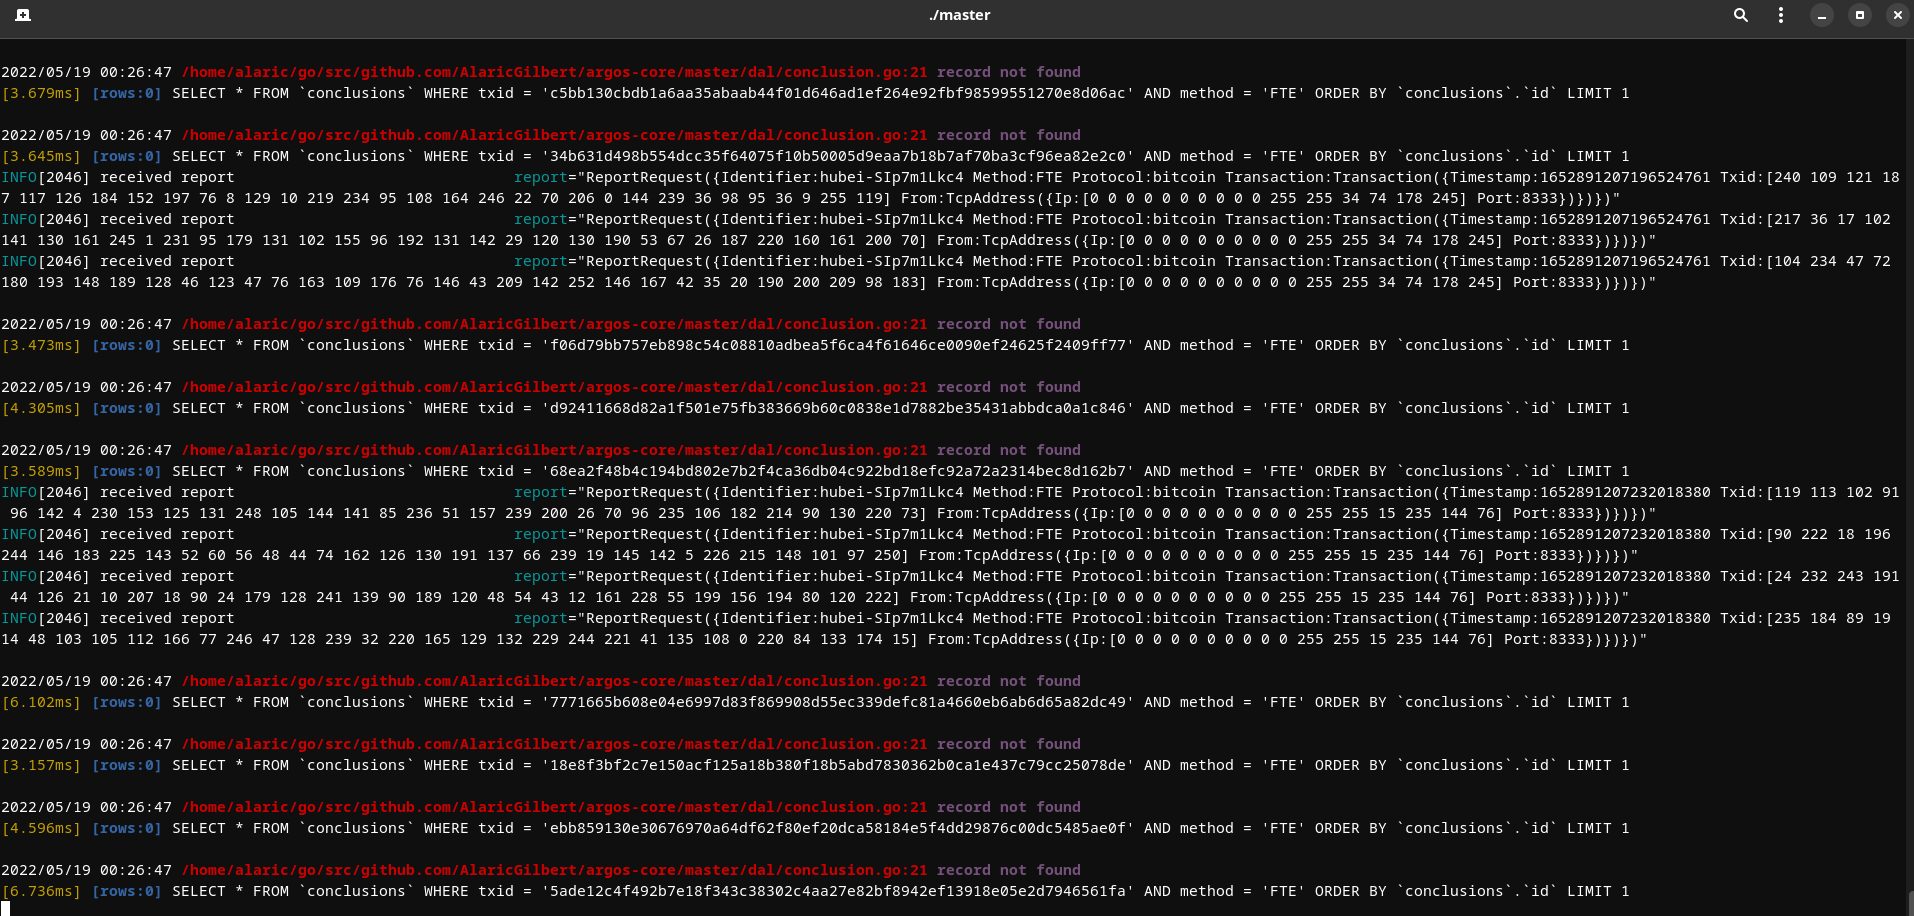
\includegraphics[width=\textwidth]{images/5.3-master.png}
}

\rfig{test:sniffer}和\rfig{test:master}表明嗅探节点运行正常,能够完成一定的对加密货币公有链交易进行监控和去匿名化;同时在后端节点中成功收到了嗅探节点的上报信息,图中“not found”的消息为在更新结论表时首先要查询,在某个交易id首次上报时查询不到是符合预期的。测试表明系统成功实现了区块链公有链的监控与溯源功能。
\subsection{客户端页面呈现}
通过点击客户端的查询按钮,即可对近段时间或指定时间段的交易进行查询。其运行情况可见\rfig{test:query}、\rfig{test:status}和\rfig{test:config}。

\xfig{test:query}{客户端按时间查询交易信息运行情况}{
  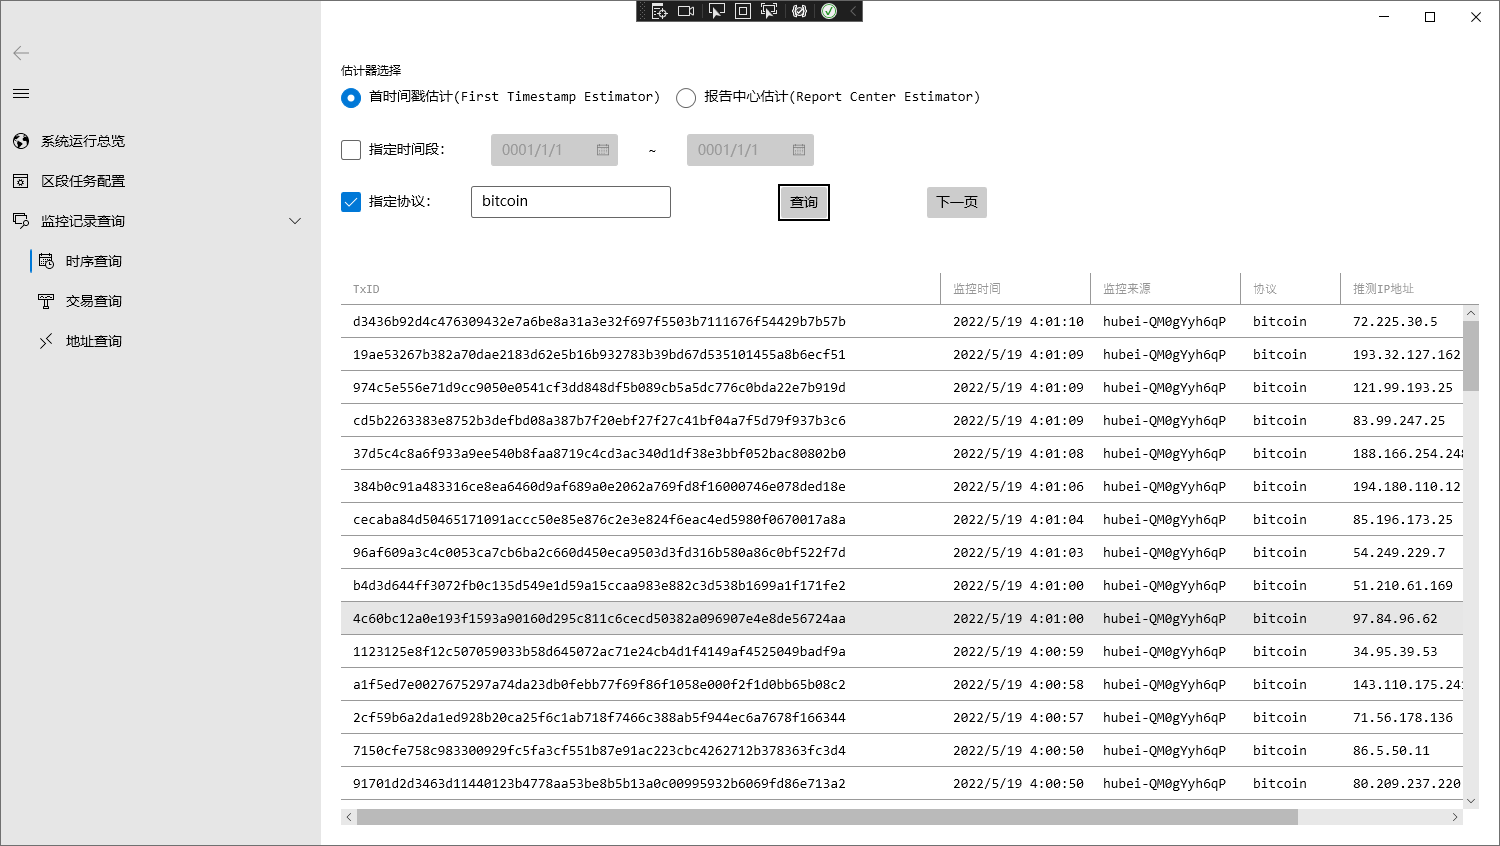
\includegraphics[width=\textwidth]{images/5.4-query.png}
}

\xfig{test:status}{客户端查看系统后端运行情况\\(折线图为按分钟平均的每秒后端收到交易信息数)}{
  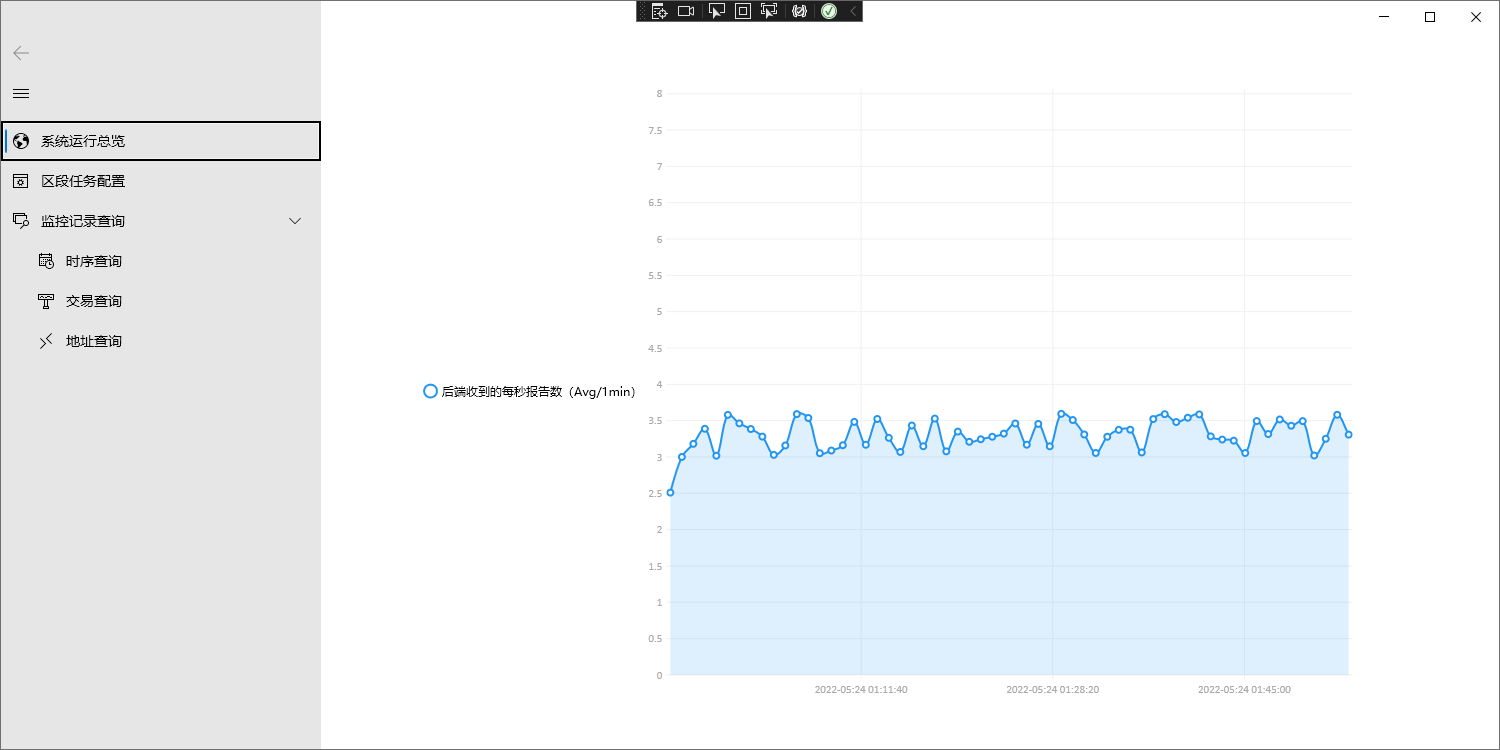
\includegraphics[width=.9\textwidth]{images/5.4-status.png}
}

\xfig{test:config}{客户端设置任务\\(尝试添加前缀为“newtest”的任务,协议为“testprotocol”)}{
  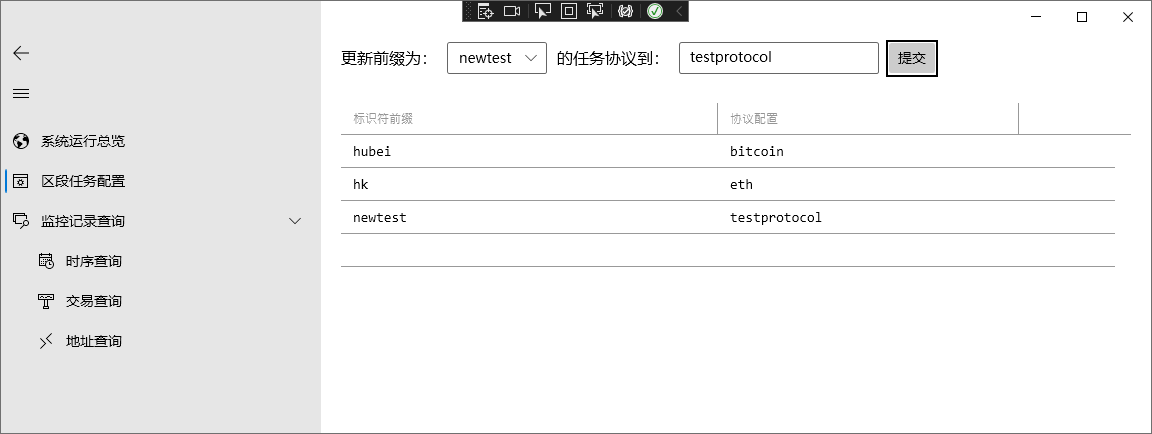
\includegraphics[width=.9\textwidth]{images/5.4-config.png}
}



\subsection{本章小结}
本章从单元测试开始,一步步由细节模块到系统整体进行了全面的测试,测试表明:系统通讯协议实现正确,能够连接入比特币等加密货币网络并获取信息;系统能够正确设置并下发不同节点的任务协议信息,能够进行多节点数据通信;系统能够利用获取的时序化网络节点信息和交易信息,对交易信息进行一定程度的去匿名化,得到其源节点IP地址,也能经客户端对获取的去匿名化的交易信息以不同的维度进行查询使用。
\newpage
\section{总结与展望}
本文从需求分析出发,经经济可行性分析和社会可行性分析后选取了合适的技术实现手段,设计并实现了一个区块链公有链交易监控与溯源系统。该系统分为功能上相对解耦合的嗅探监控、后端存储和客户端操作展示三大模块和耦合在嗅探监控模块中的以比特币协议作为实现范例的加密货币通信托管模块。经测试后表明系统具有监控区块链公有链上交易信息发生并对其进行一定的去匿名化分析的能力,在一定程度上改善了加密货币缺乏系统性监控溯源工具的现状,为国家安全部门和金融监管机构提供了一定的去匿名化追踪解决方案。

本文设计的系统有较好的拓展性,可以轻松地在系统提供的接口上进行扩展实现更多加密货币的协议和监控的算法,为实现建立更完善的加密货币监管系统提供了一种解决思路。但本系统目前仅支持了比特币一种加密货币,也只使用了两种方式对其交易进行去匿名化,仍有相当的改进空间,下一步的工作将从以下方面进行:

(1)\textbf{实现更多的加密货币通信协议}\ 目前得到广泛应用的加密货币除了比特币,还有以太坊、莱特币等等,仅仅实现一种加密货币对于一个监控系统并不足以监控足量数据,对可能的违法犯罪行为和灰色产业的监控不够有力,需要实现更多的加密货币通信协议来完善;

(2)\textbf{增强对于NAT\footnote{Network Address Translation,中文名网络地址转换(也称网络掩蔽、IP掩蔽)。在计算机网络中是一种在IP数据包通过路由器或防火墙时重写来源IP地址或目的IP地址的技术。这种技术被普遍使用在有多台主机但只通过一个公有IP地址访问互联网的私有网络中。是一个方便且得到了广泛应用的技术。}网络后的节点的监控}\ 由于无法建立到经NAT后的节点的TCP连接,无法目前系统尚不能直接处理得到处于NAT系统后的节点的信息,需要实现基于类似Biryukov\cite{biryukov2014deanonymisation}等人利用比特币对等网络中节点发现的协议的方法处理得到入口节点的方式来实现NAT网络后的节点的监控。

(3)\textbf{增强用户与权限系统}\ 目前系统缺乏用户与权限系统,部署后保证安全需要使后端HTTP接口仅在同一网段访问,以保障系统数据的安全;需要增加用户权限系统,对HTTP接口权限进行校验,同时对任务的配置修改、用户导入进行鉴权,增加不同用户组保障工作人员操作上的安全性和合法性。


\begin{thankpage}

本次毕业设计从二月到五月共计快四个月的时间,是本人完成的非纯业务性系统中最复杂的一个,极大地锻炼了我分析到解决复杂性问题和信息资料检索的能力。在完成毕业设计的过程中受到了许多帮助,本人不胜感激。

首先感谢赐予我生命并养育我成人的父母,是他们给了我来到这个世界上的机会,让我能有机会学习和思考;在毕业设计中我倍感憔悴的时候,是父母的鼓励让我有了继续的动力。

随即感谢我的导师XXX,感谢设计了本课题,让我度过了大学生活中最充实的一段时光,同时感谢他对设计和实现系统中给出的辛勤指导。

最后对其他在设计中给出帮助的人一并感谢:感谢室友XXX帮助解决在使用\LaTeX 过程中遇到的部分问题;感谢室友XX和XXX在比特币协议二进制解析性能优化方面提出的建议;感谢XXX同学在本设计进度安排方面提供的建议。

\end{thankpage}

\nocite{*}
\bibliography{paper}

\end{document}
